\documentclass{article}
\usepackage[a4paper,left=3cm,right=3cm,top=3cm,bottom=3cm]{geometry}
\usepackage[utf8]{inputenc}
\usepackage[T1]{fontenc}
\usepackage{latexsym,amsfonts,amsmath,amssymb,amstext,graphicx,titlesec,ae,aecompl,mathtools,tabularx, multirow, cancel, nicefrac,subcaption, blindtext, floatrow}
\setlength{\parindent}{0pt}
\newfloatcommand{capbtabbox}{table}[][\FBwidth]


\begin{document}

\begin{titlepage}
       \begin{center}
             \begin{huge}
				   %% Update assignment number here
                   \textbf{Assignment 5}
             \end{huge}
       \end{center}

       \begin{center}
             \begin{large}
                   Computational Intelligence, SS2020
             \end{large}
       \end{center}

       \begin{center}
 \begin{tabularx}{\textwidth}{|>{\hsize=.33\hsize}X|>{\hsize=.33\hsize}X|>{\hsize=.33\hsize}X|} 

                   \hline
                   \multicolumn{3}{|c|}{\textbf{Team Members}} \\
                   \hline
                   Last name & First name & Matriculation Number \\
                   \hline
                   Blöcher & Christian & 01573246 \\
                   \hline
                   Bürgener & Max & 01531577 \\
                   \hline
                    &  &  \\
                   \hline

             \end{tabularx}
       \end{center}
\end{titlepage}


\section{Classification - 2 dimensional feature}
\subsection{EM algorithm}

\begin{figure}[!ht]
	\makebox[\textwidth]{
	\begin{subfigure}{0.6\textwidth}
	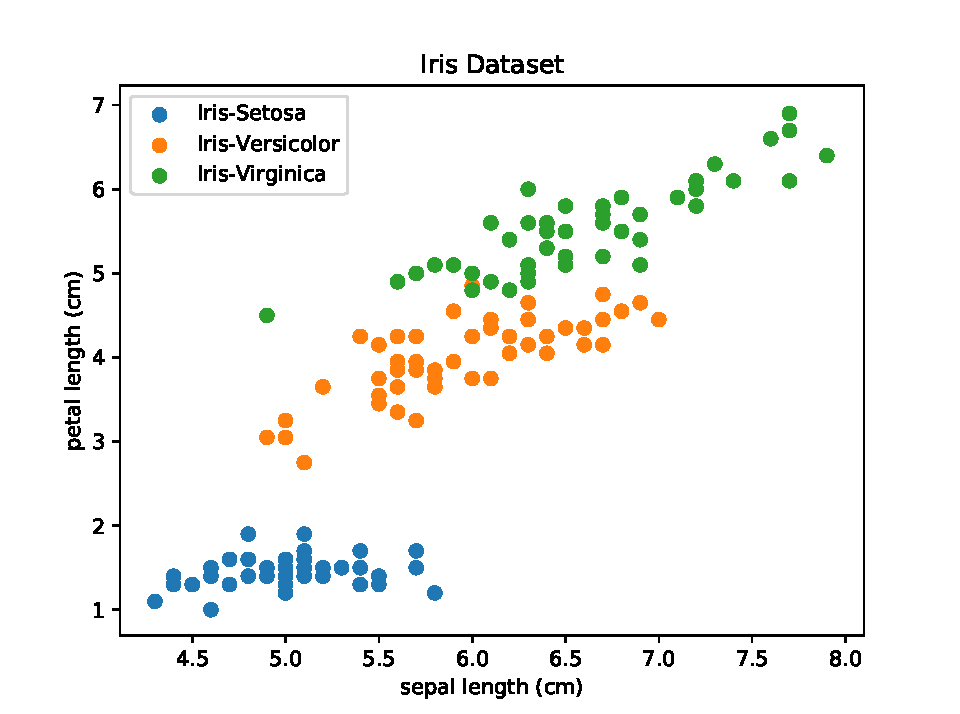
\includegraphics[width=\textwidth]{./Figures/data}
	%\caption{Dataset}
	\end{subfigure}
	\begin{subfigure}{0.6\textwidth}
	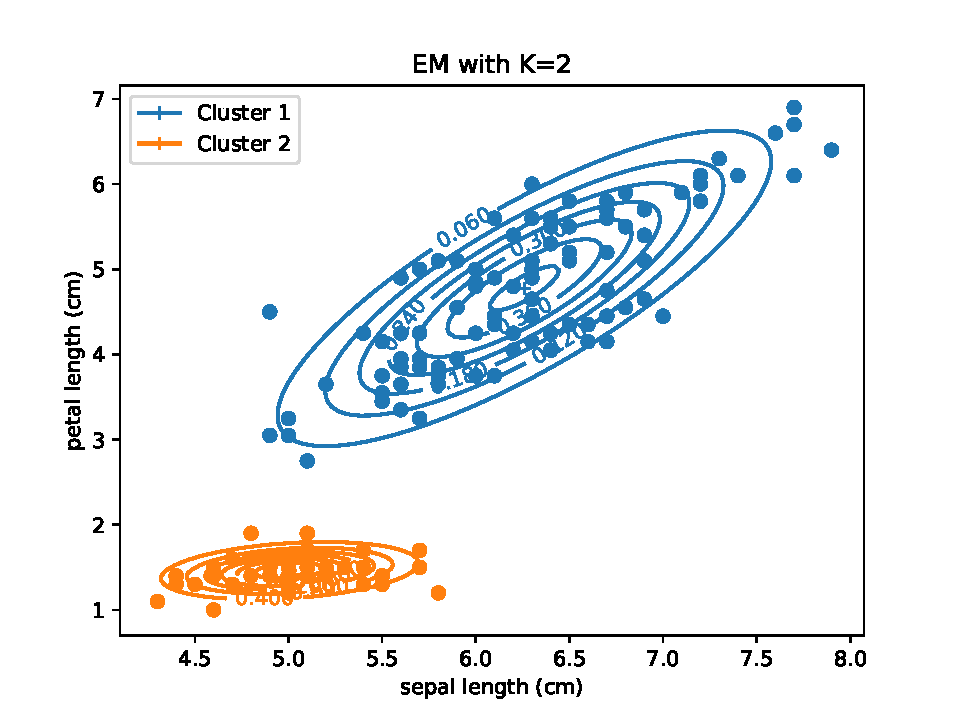
\includegraphics[width=\textwidth]{./Figures/2_1_EM_cont_K2}
	%\caption{$K=2$}
	\end{subfigure}
	}
	\makebox[\textwidth]{
	\begin{subfigure}{0.6\textwidth}
	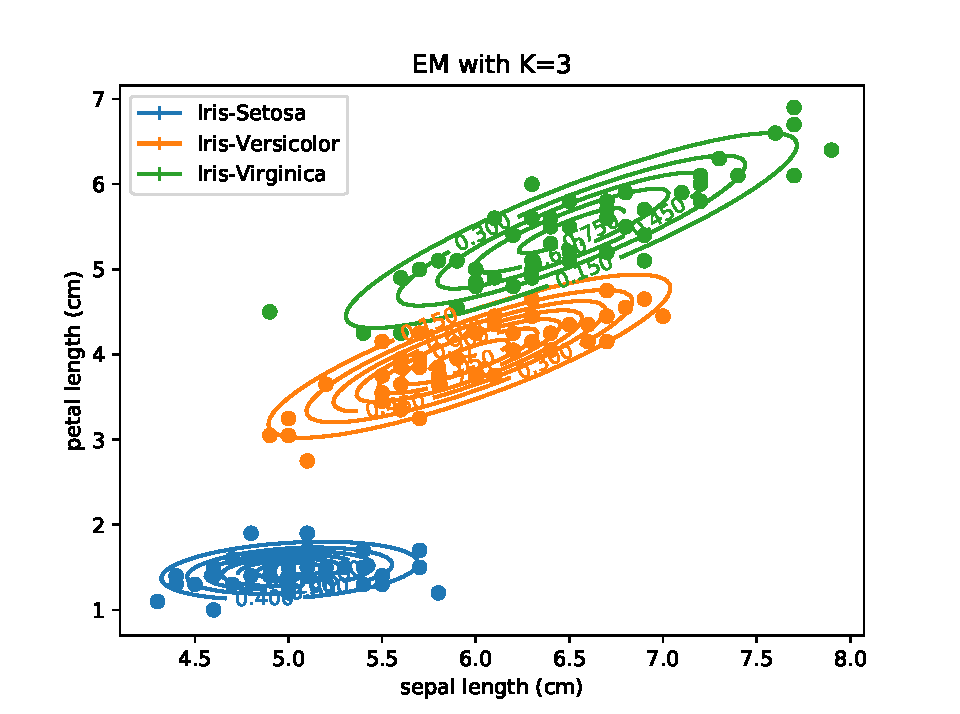
\includegraphics[width=\textwidth]{./Figures/2_1_EM_cont_K3}
	%\caption{$K=3$}
	\end{subfigure}
	\begin{subfigure}{0.6\textwidth}
	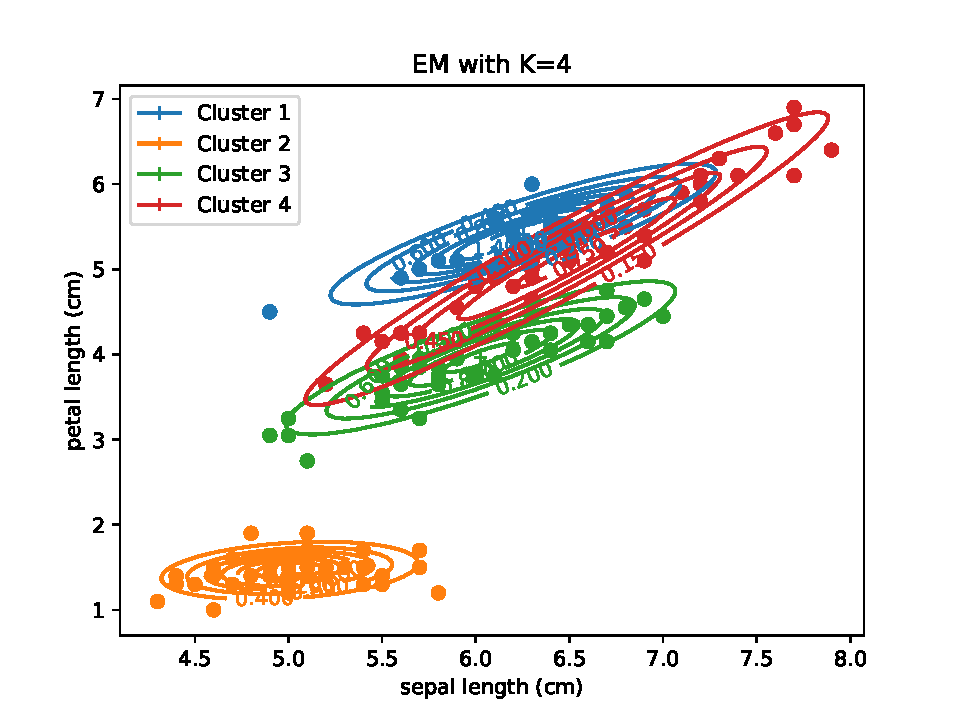
\includegraphics[width=\textwidth]{./Figures/2_1_EM_cont_K4}
	%\caption{$K=4$}
	\end{subfigure}
	}	
	\caption{Results of EM classification with $K=2\dots4$ components.}
	\label{2_1_EM_cont}
\end{figure}

\begin{figure}[!ht]
\centering
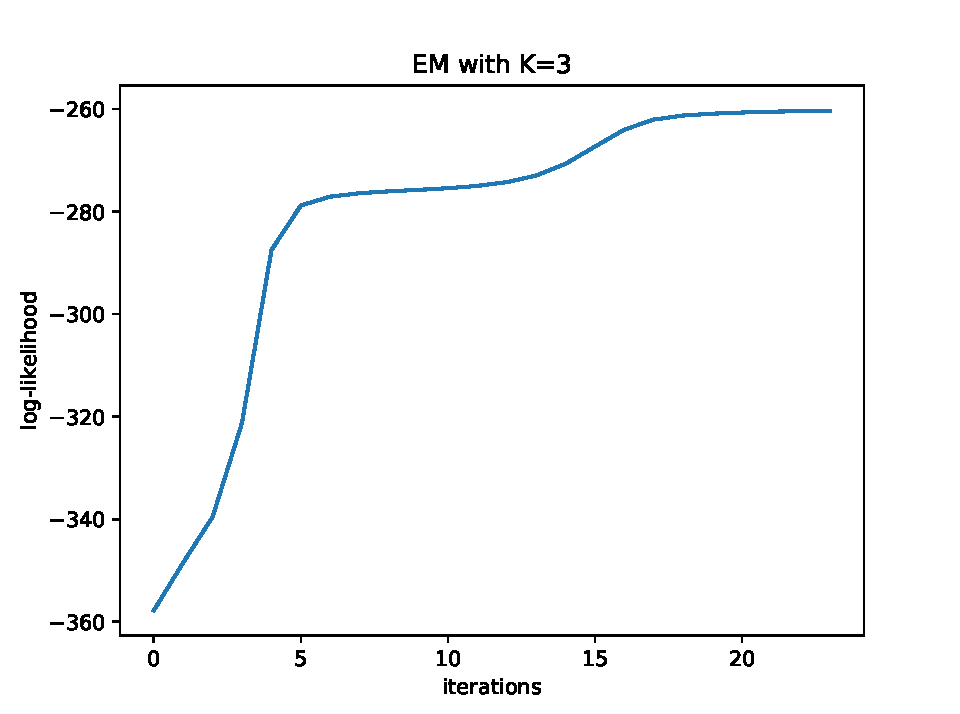
\includegraphics[width=0.6\textwidth]{./Figures/2_1_EM_likelihood_K3}
\caption{Log-likelihood function over iterations for $K=3$ components.}
\label{2_1_EM_likelihood}
\end{figure}

\begin{figure}[!ht]
	\makebox[\textwidth]{
	\begin{subfigure}{0.6\textwidth}
	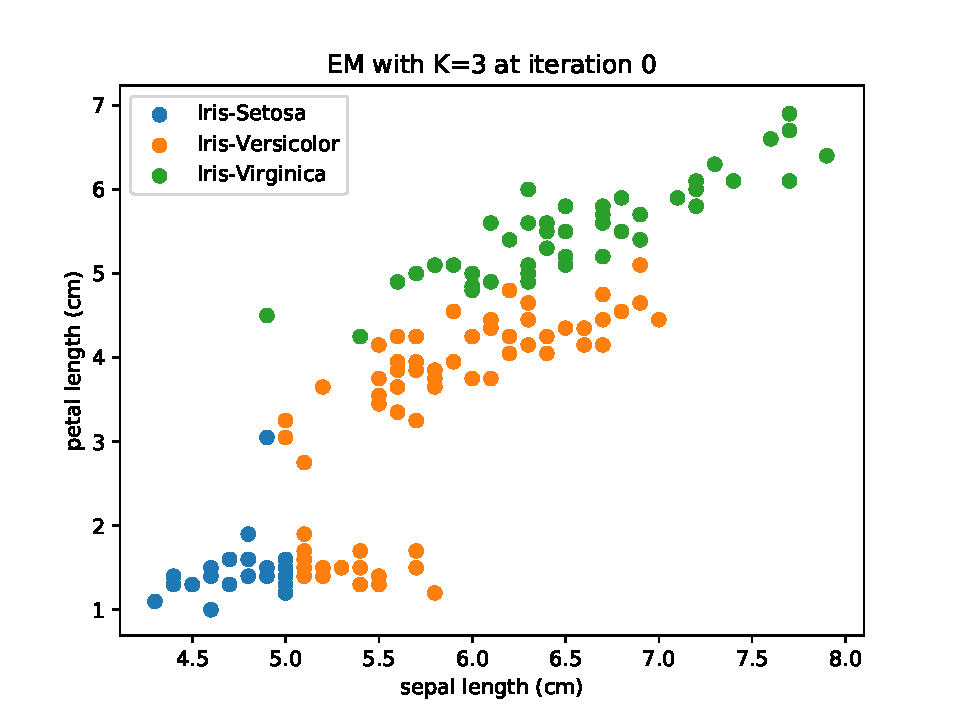
\includegraphics[width=\textwidth]{./Figures/2_1_EM_iter0}
	%\caption{Dataset}
	\end{subfigure}
	\begin{subfigure}{0.6\textwidth}
	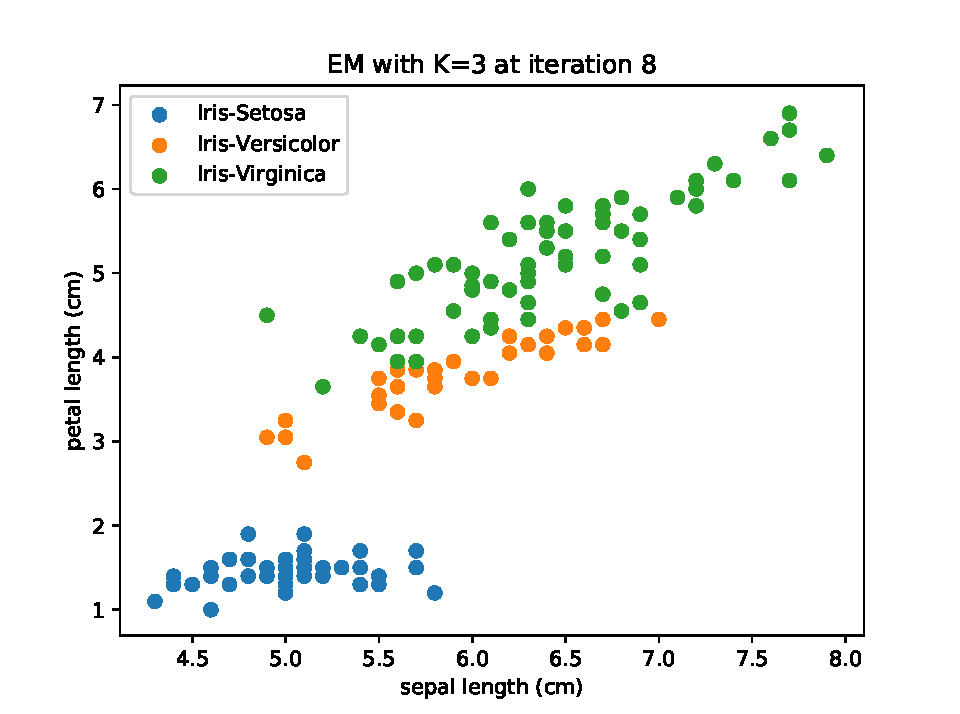
\includegraphics[width=\textwidth]{./Figures/2_1_EM_iter8}
	%\caption{$K=2$}
	\end{subfigure}
	}
	\makebox[\textwidth]{
	\begin{subfigure}{0.6\textwidth}
	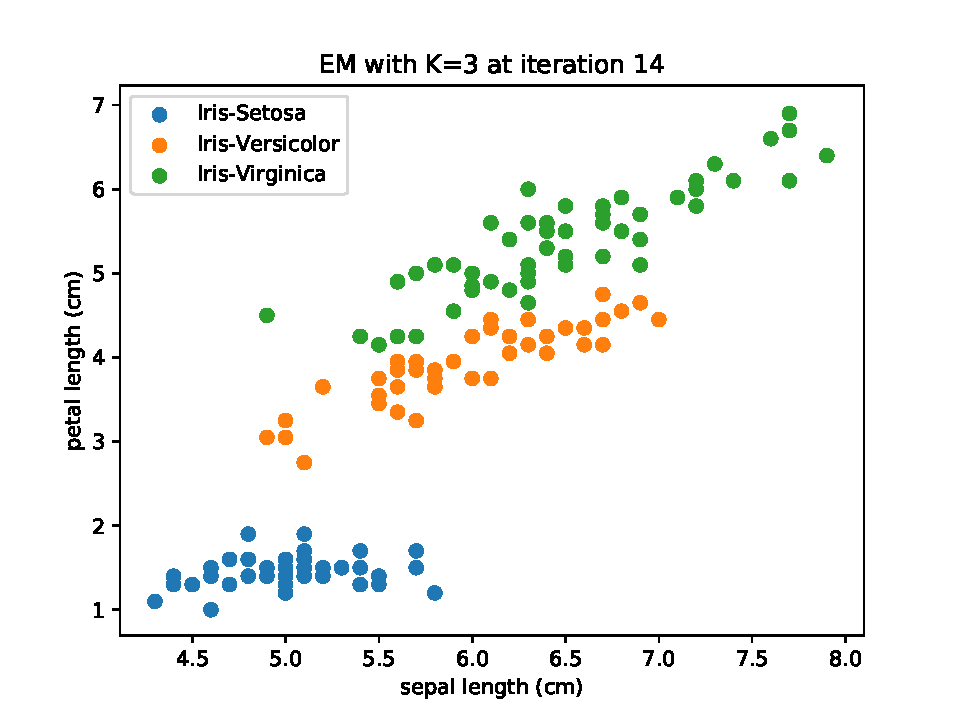
\includegraphics[width=\textwidth]{./Figures/2_1_EM_iter14}
	%\caption{$K=3$}
	\end{subfigure}
	\begin{subfigure}{0.6\textwidth}
	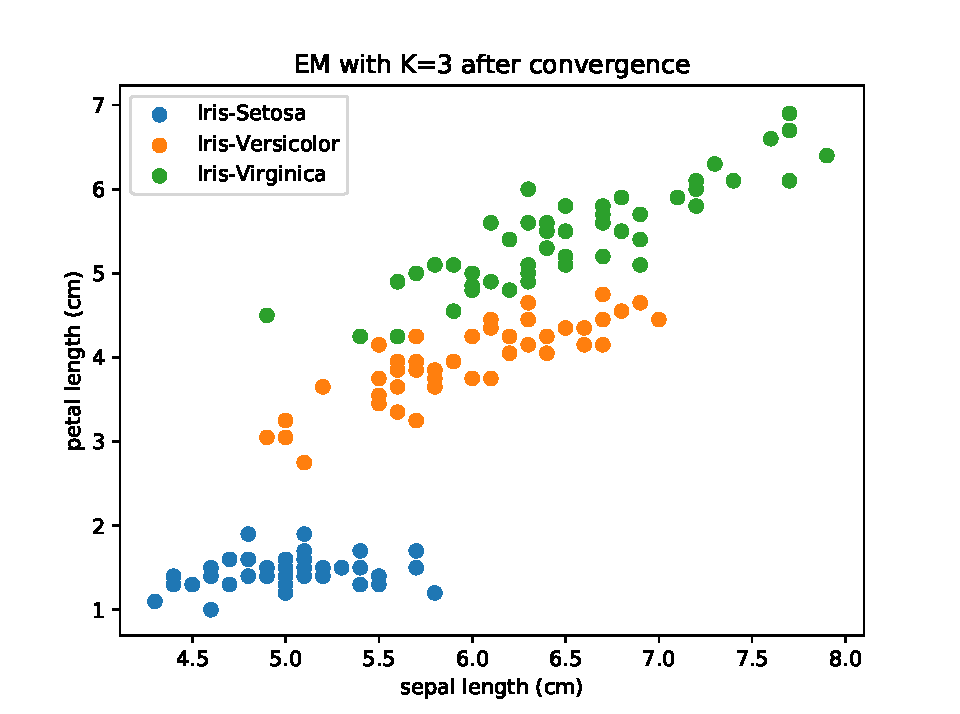
\includegraphics[width=\textwidth]{./Figures/2_1_EM_converged}
	%\caption{$K=4$}
	\end{subfigure}
	}	
	\caption{Results of soft-classification done in E-step.}
	\label{2_1_EM_iter}
\end{figure}


\begin{figure}[!ht]
	\makebox[\textwidth]{
	\begin{subfigure}{0.6\textwidth}
	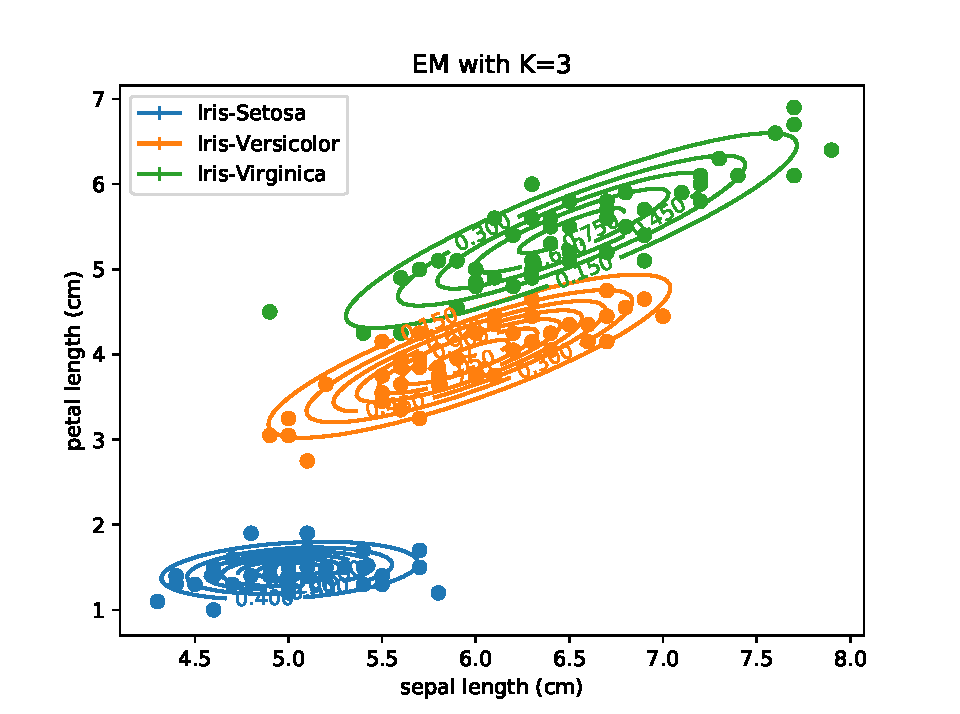
\includegraphics[width=\textwidth]{./Figures/2_1_EM_cont_K3}
	%\caption{Dataset}
	\end{subfigure}
	\begin{subfigure}{0.6\textwidth}
	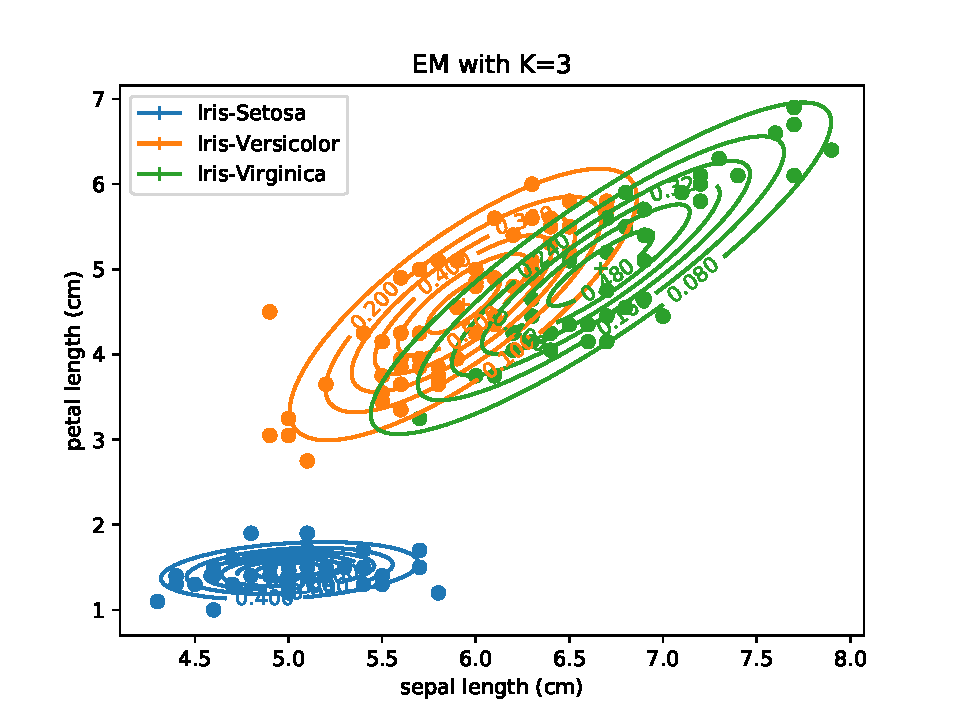
\includegraphics[width=\textwidth]{./Figures/2_1_EM_randinit1}
	%\caption{$K=2$}
	\end{subfigure}
	}
	\makebox[\textwidth]{
	\begin{subfigure}{0.6\textwidth}
	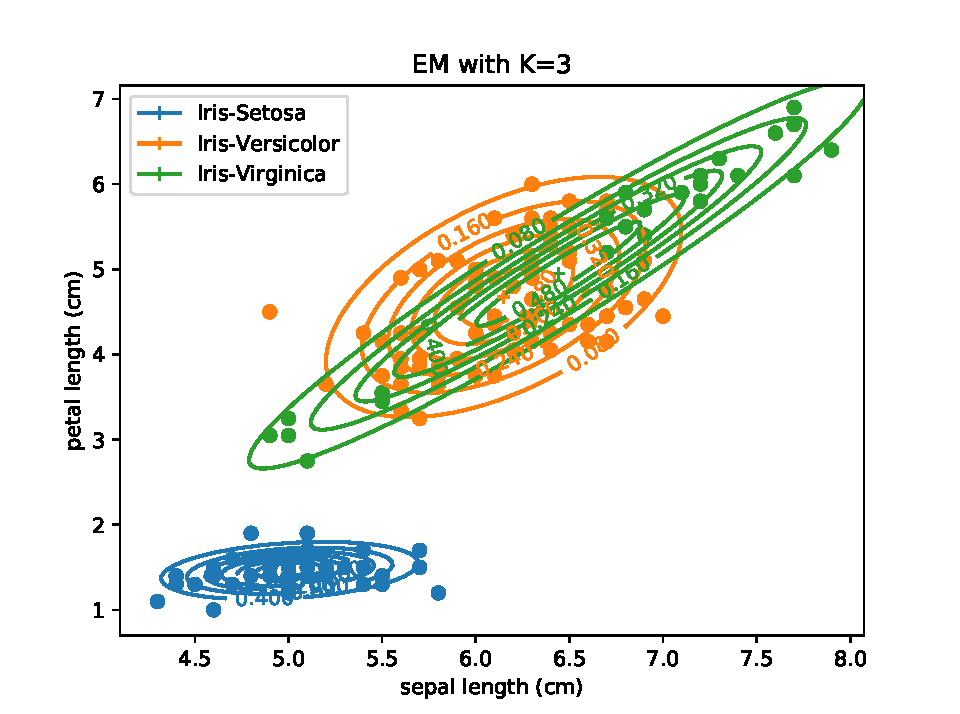
\includegraphics[width=\textwidth]{./Figures/2_1_EM_randinit2}
	%\caption{$K=3$}
	\end{subfigure}
	\begin{subfigure}{0.6\textwidth}
	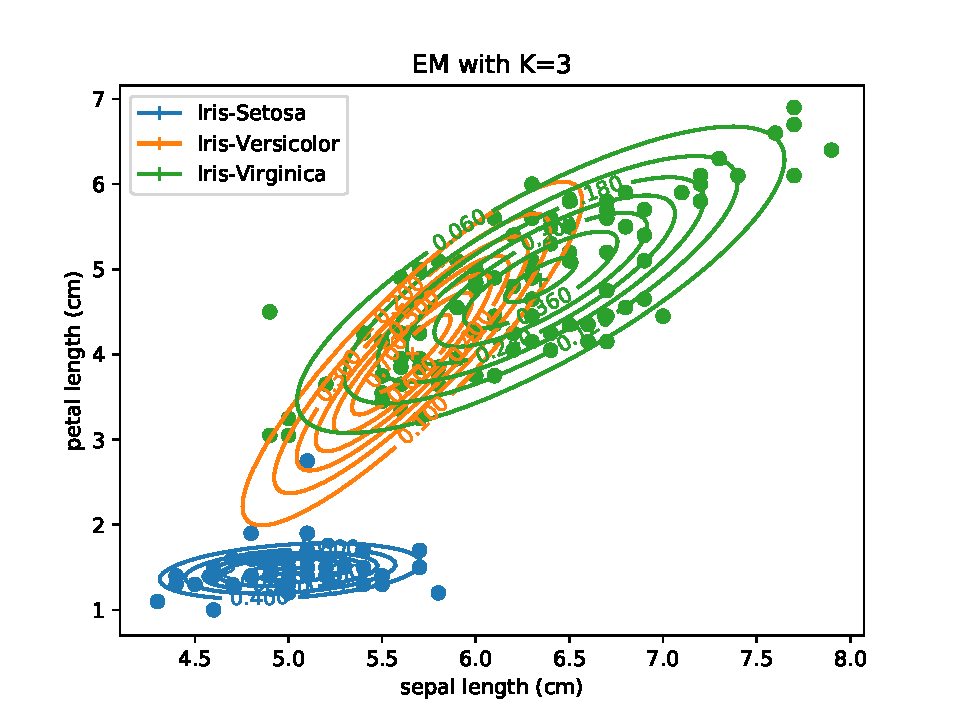
\includegraphics[width=\textwidth]{./Figures/2_1_EM_randinit3}
	%\caption{$K=4$}
	\end{subfigure}
	}	
	\caption{Results of EM classification for several random \texttt{mean0} starting samples.}
	\label{2_1_EM_randinit}
\end{figure}

\clearpage

\subsection{K-means algorithm}

\begin{figure}[!ht]
	\makebox[\textwidth]{
	\begin{subfigure}{0.6\textwidth}
	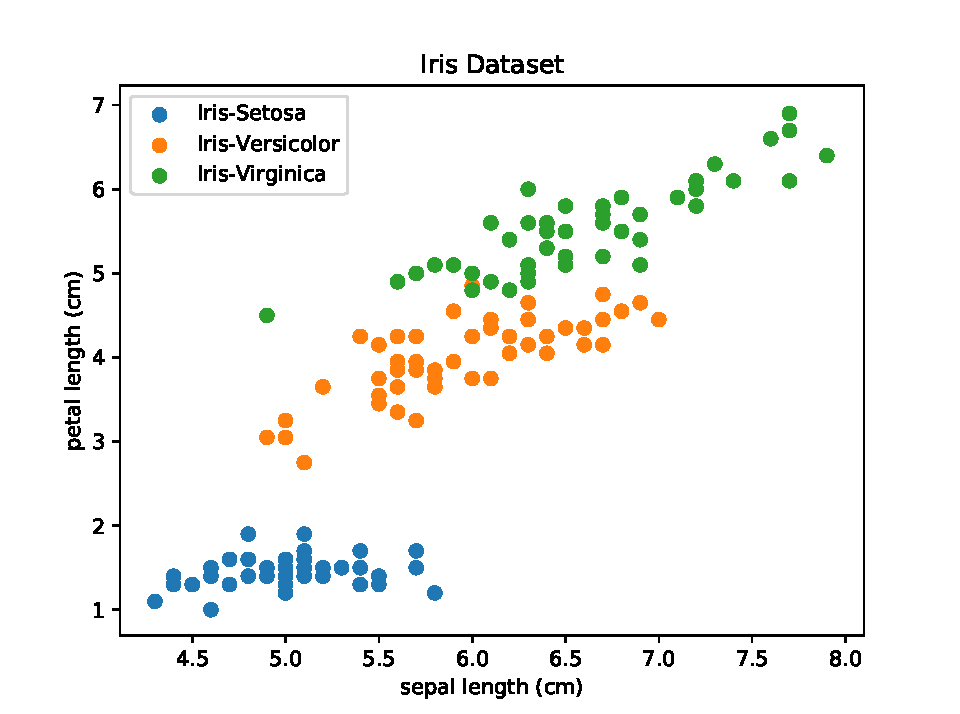
\includegraphics[width=\textwidth]{./Figures/data}
	%\caption{Dataset}
	\end{subfigure}
	\begin{subfigure}{0.6\textwidth}
	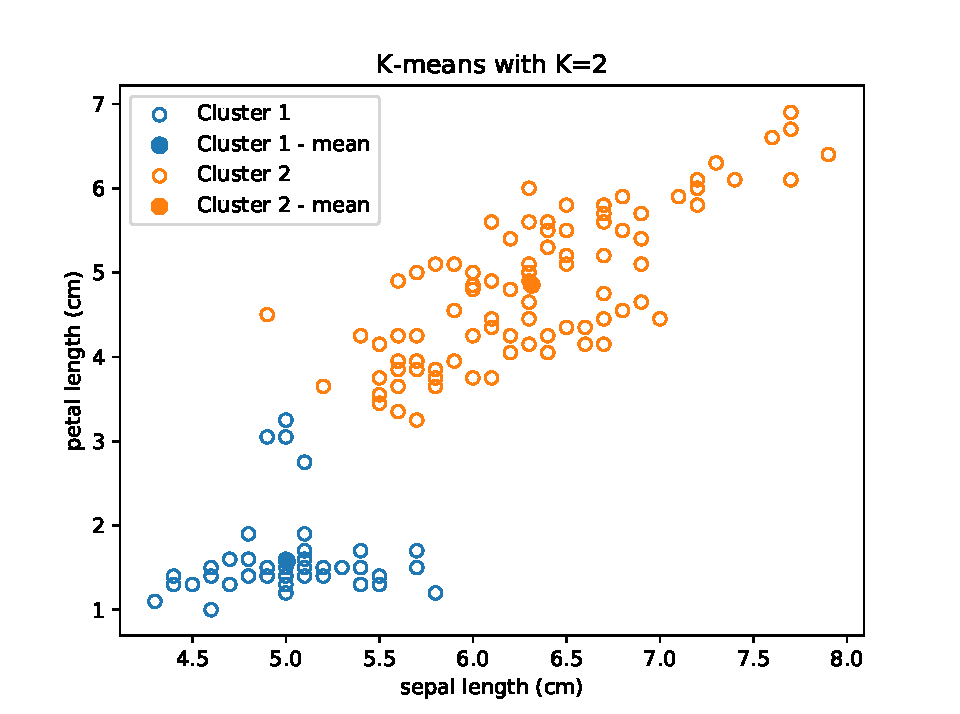
\includegraphics[width=\textwidth]{./Figures/2_1_Kmeans_scatter_K2}
	%\caption{$K=2$}
	\end{subfigure}
	}
	\makebox[\textwidth]{
	\begin{subfigure}{0.6\textwidth}
	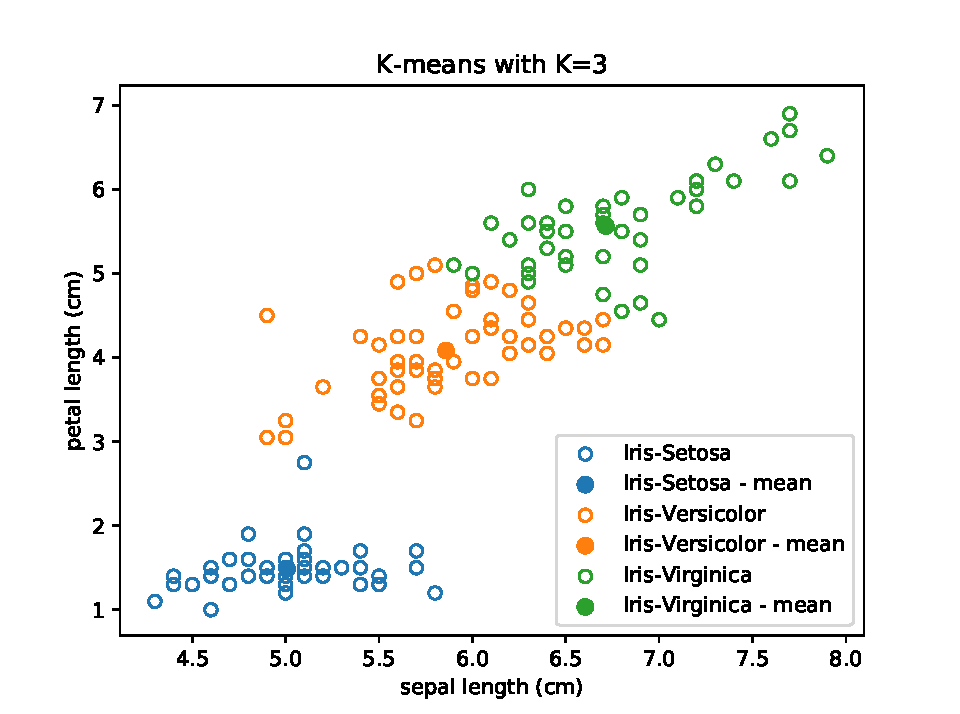
\includegraphics[width=\textwidth]{./Figures/2_1_Kmeans_scatter_K3}
	%\caption{$K=3$}
	\end{subfigure}
	\begin{subfigure}{0.6\textwidth}
	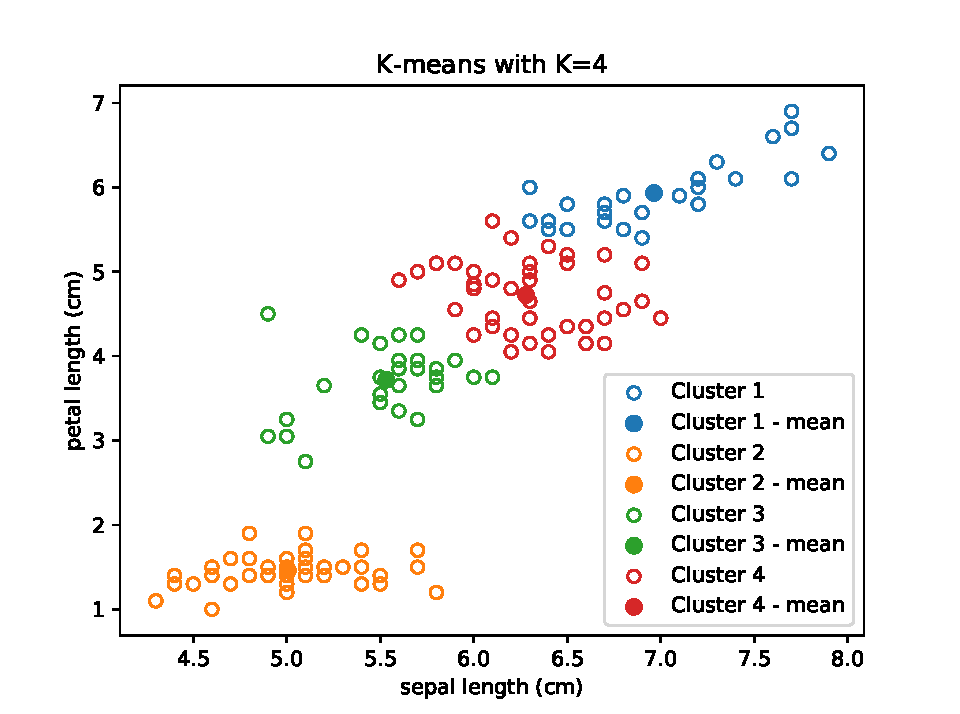
\includegraphics[width=\textwidth]{./Figures/2_1_Kmeans_scatter_K4}
	%\caption{$K=4$}
	\end{subfigure}
	}	
	\caption{Results of K-means classification with $K=2\dots4$ components.}
	\label{2_1_Kmeans_scatter}
\end{figure}

\begin{figure}[!ht]
\centering
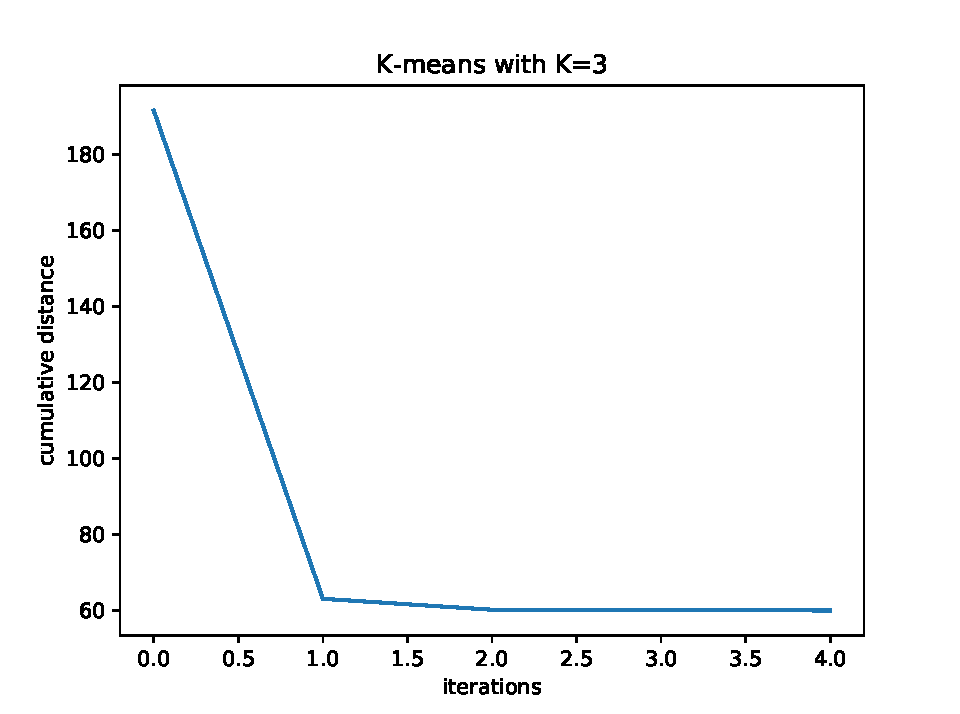
\includegraphics[width=0.6\textwidth]{./Figures/2_1_Kmeans_distance_K3}
\caption{Cumulative distance function over iterations for $K=3$ components.}
\label{2_1_Kmeans_distance}
\end{figure}

The classification using K-means algorithm is also good. But in comparison to the EM-algorithm outliers are more often misclassified. The additional 4th cluster adds another classification area which can be clearly distinguished from all others, since all datapoints are spherically gathered around the mean value.
The cumulative distance quickly converges after one iteration. 
 
\begin{figure}[!ht]
	\makebox[\textwidth]{
	\begin{subfigure}{0.6\textwidth}
	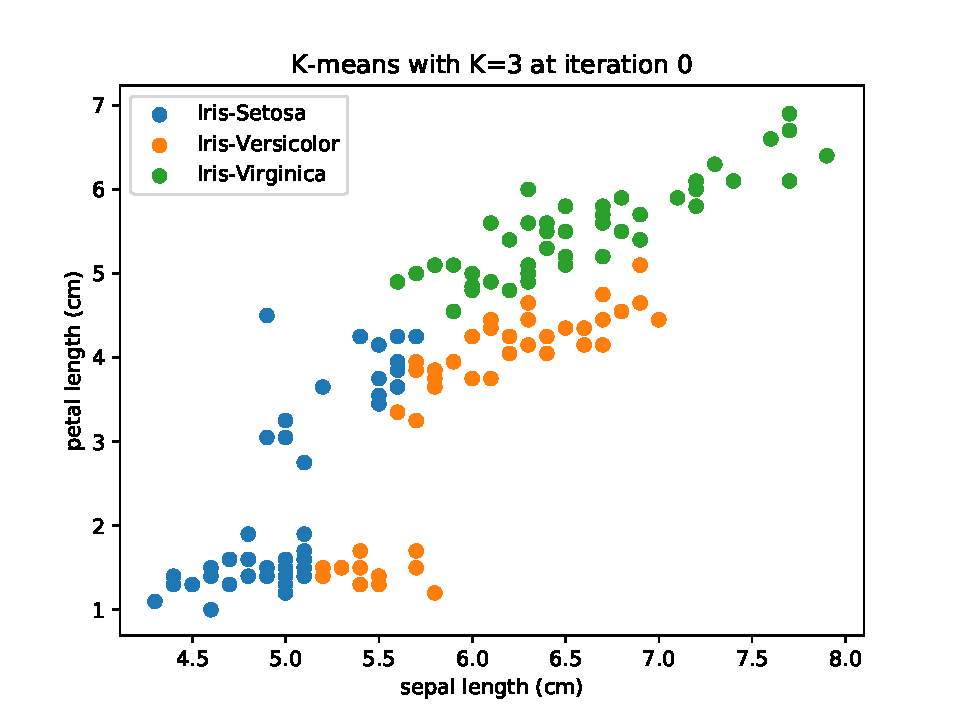
\includegraphics[width=\textwidth]{./Figures/2_1_Kmeans_iter0}
	%\caption{Dataset}
	\end{subfigure}
	\begin{subfigure}{0.6\textwidth}
	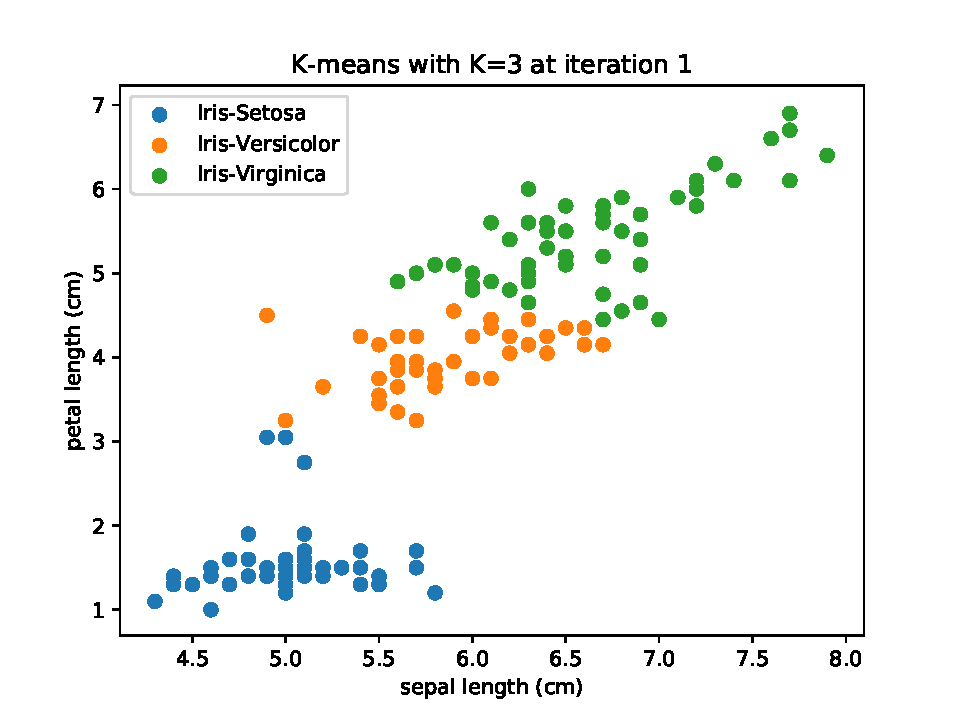
\includegraphics[width=\textwidth]{./Figures/2_1_Kmeans_iter1}
	%\caption{$K=2$}
	\end{subfigure}
	}
	\makebox[\textwidth]{
	\begin{subfigure}{0.6\textwidth}
	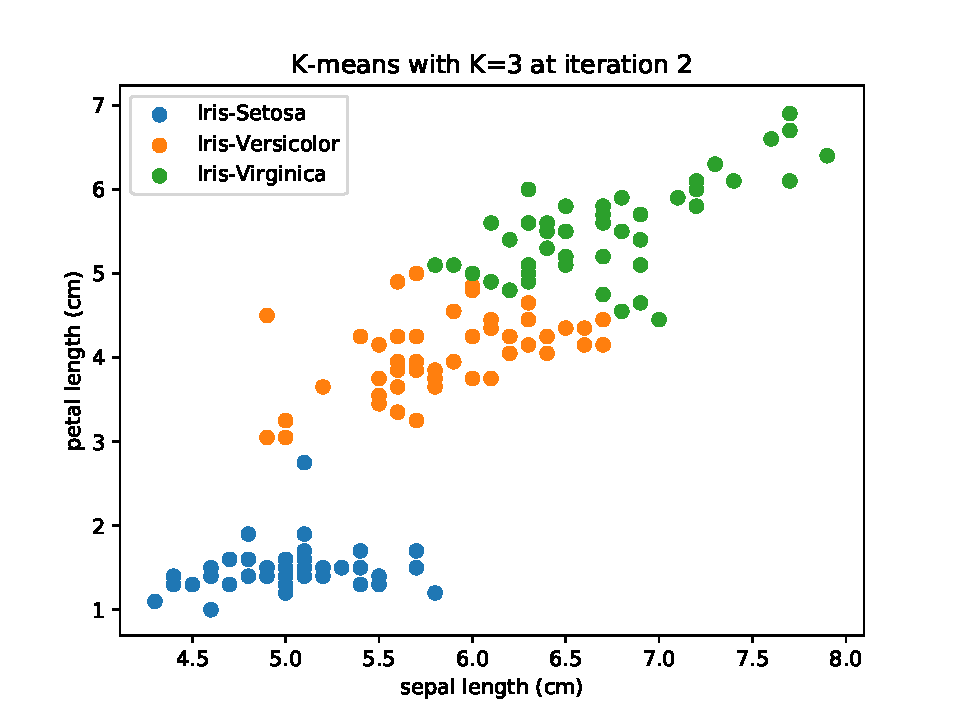
\includegraphics[width=\textwidth]{./Figures/2_1_Kmeans_iter2}
	%\caption{$K=3$}
	\end{subfigure}
	\begin{subfigure}{0.6\textwidth}
	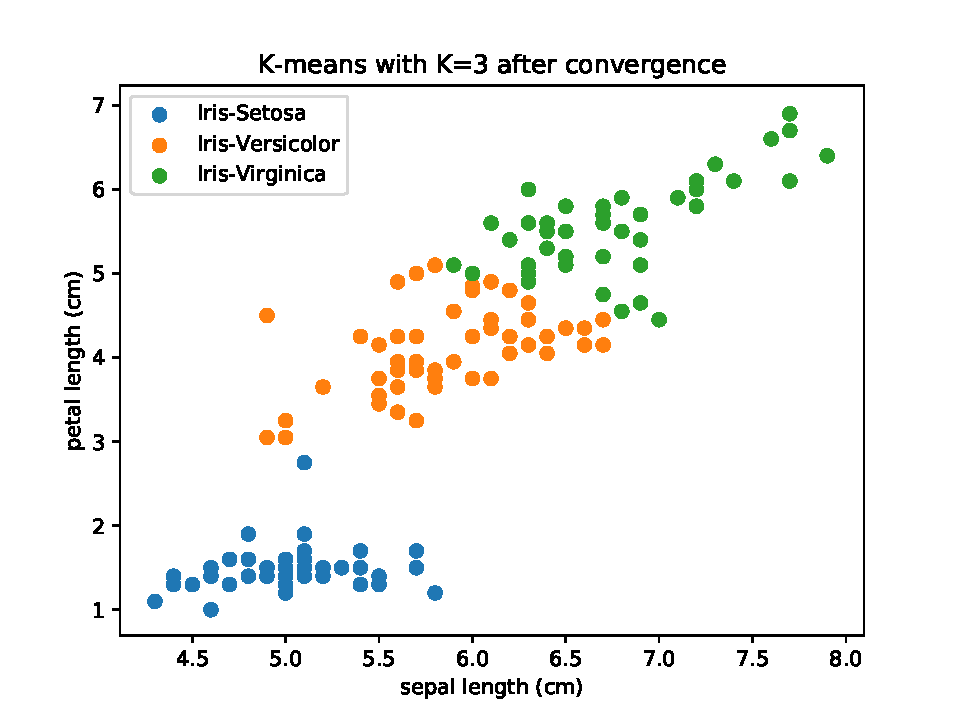
\includegraphics[width=\textwidth]{./Figures/2_1_Kmeans_converged}
	%\caption{$K=4$}
	\end{subfigure}
	}	
	\caption{Results of hard-classification during optimisation.}
	\label{2_1_Kmeans_iter}
\end{figure}

The classification results are getting better with more iterations. This makes sense, since the start mean values are randomly initialized and new calculated for each iteration.
\newpage
\begin{figure}[!ht]
	\makebox[\textwidth]{
	\begin{subfigure}{0.6\textwidth}
	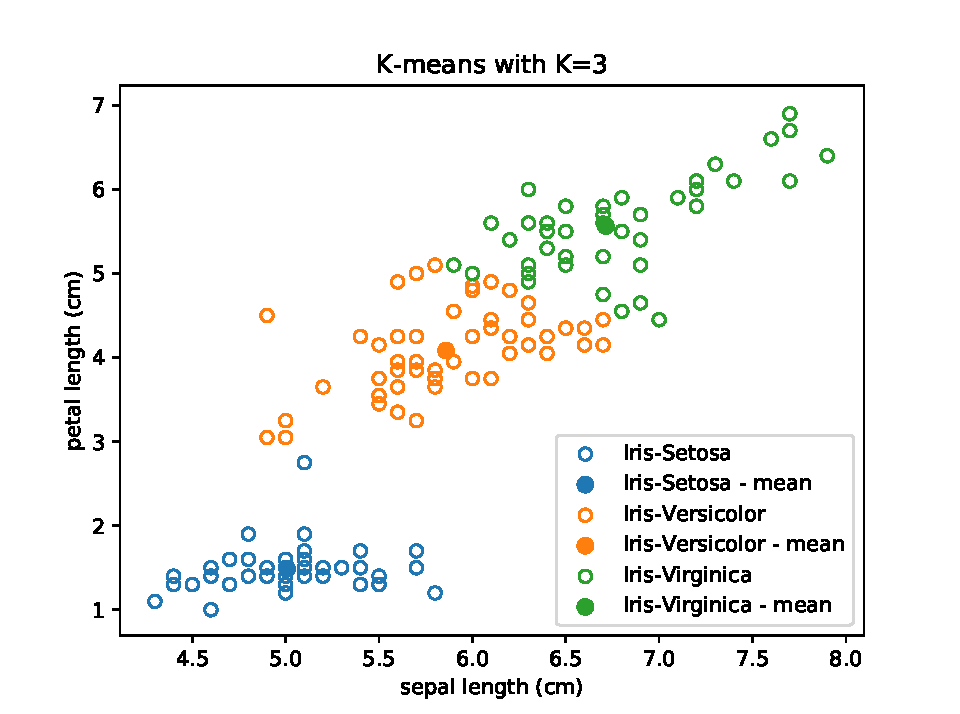
\includegraphics[width=\textwidth]{./Figures/2_1_Kmeans_scatter_K3}
	%\caption{Dataset}
	\end{subfigure}
	\begin{subfigure}{0.6\textwidth}
	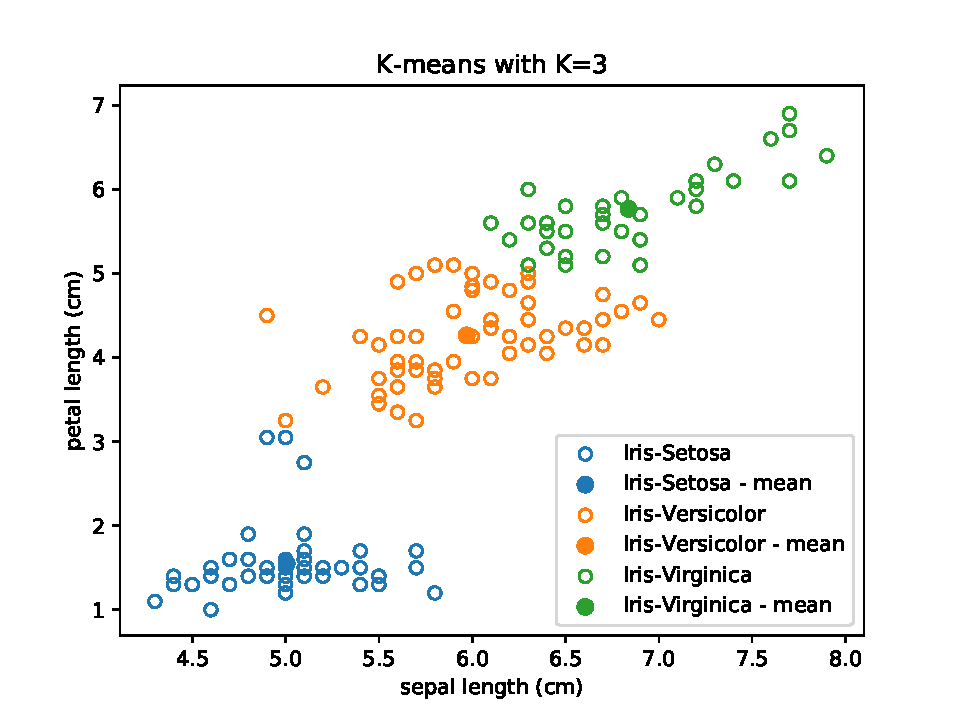
\includegraphics[width=\textwidth]{./Figures/2_1_Kmeans_randinit1}
	%\caption{$K=2$}
	\end{subfigure}
	}
	\makebox[\textwidth]{
	\begin{subfigure}{0.6\textwidth}
	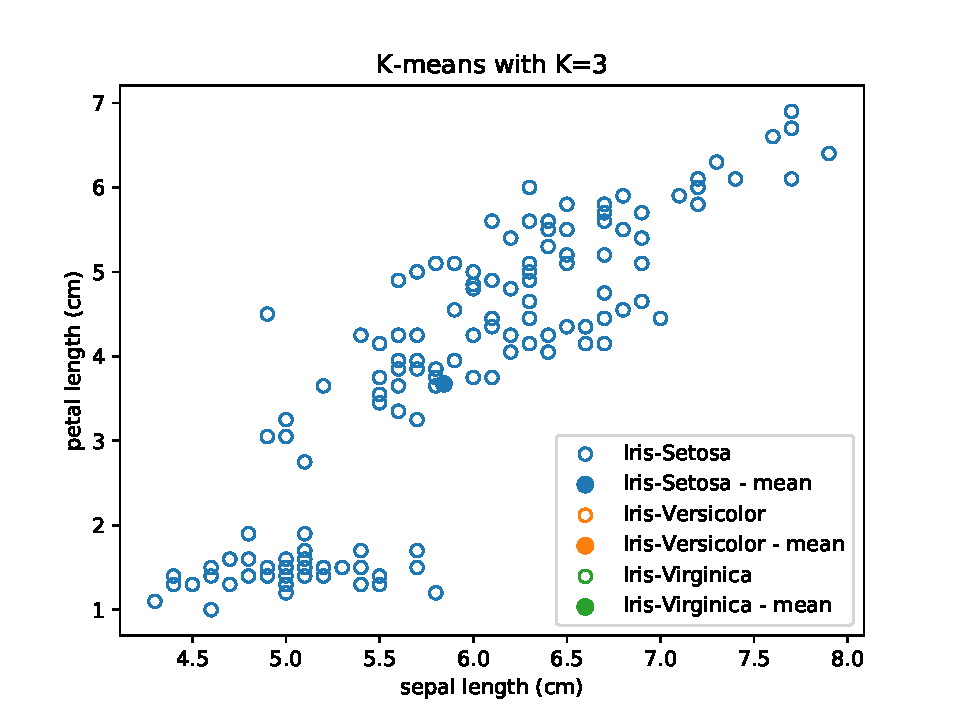
\includegraphics[width=\textwidth]{./Figures/2_1_Kmeans_randinit2}
	%\caption{$K=3$}
	\end{subfigure}
	\begin{subfigure}{0.6\textwidth}
	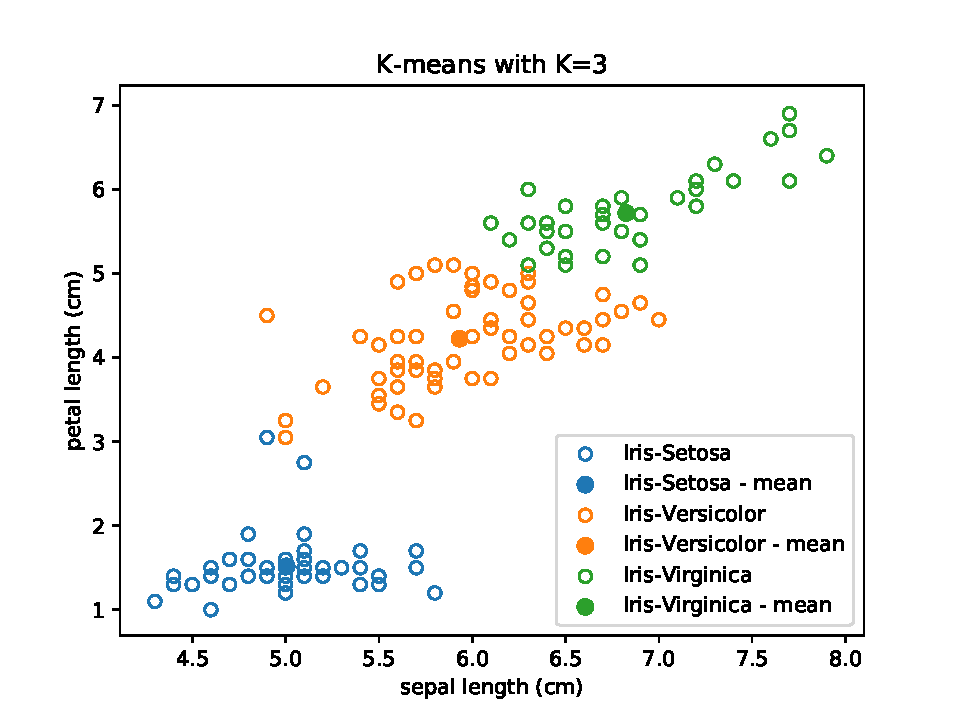
\includegraphics[width=\textwidth]{./Figures/2_1_Kmeans_randinit3}
	%\caption{$K=4$}
	\end{subfigure}
	}	
	\caption{Results of K-means classification for several random \texttt{center0} starting samples.}
	\label{2_1_Kmeans_randinit}
\end{figure}

Figure \ref{2_1_Kmeans_randinit} supports our assumption that the algorithm is prone to misclassify outliers. The algorithm also seems to have problems with not clearly separated clusters because a lot data samples were misclassified at the border of "Iris-Versicolor" and "Iris-Virginica".

\clearpage

\section{Classification - 4 dimensional feature}
\subsection{EM algorithm}

\begin{figure}[!ht]
	\makebox[\textwidth]{
	\begin{subfigure}{0.6\textwidth}
	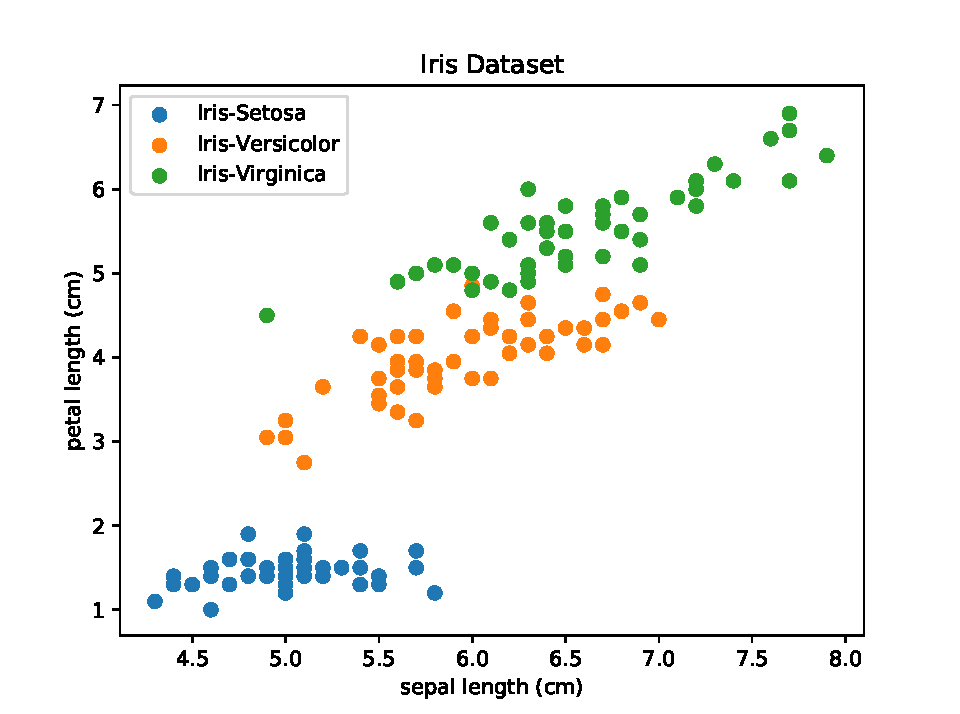
\includegraphics[width=\textwidth]{./Figures/data}
	%\caption{Dataset}
	\end{subfigure}
	\begin{subfigure}{0.6\textwidth}
	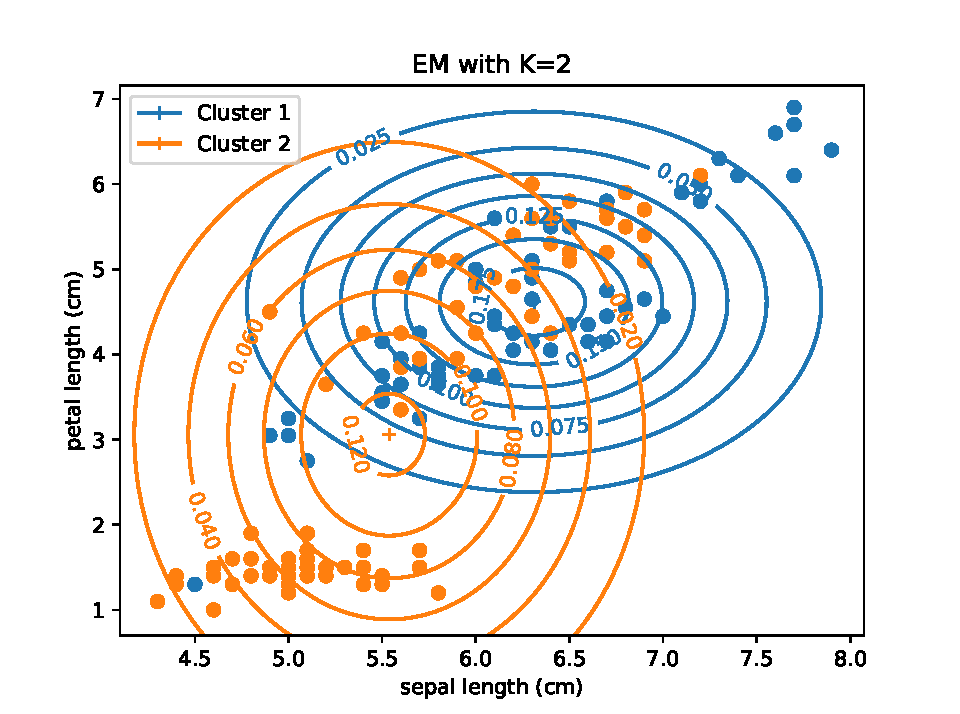
\includegraphics[width=\textwidth]{./Figures/2_2_EM_cont_K2}
	%\caption{$K=2$}
	\end{subfigure}
	}
	\makebox[\textwidth]{
	\begin{subfigure}{0.6\textwidth}
	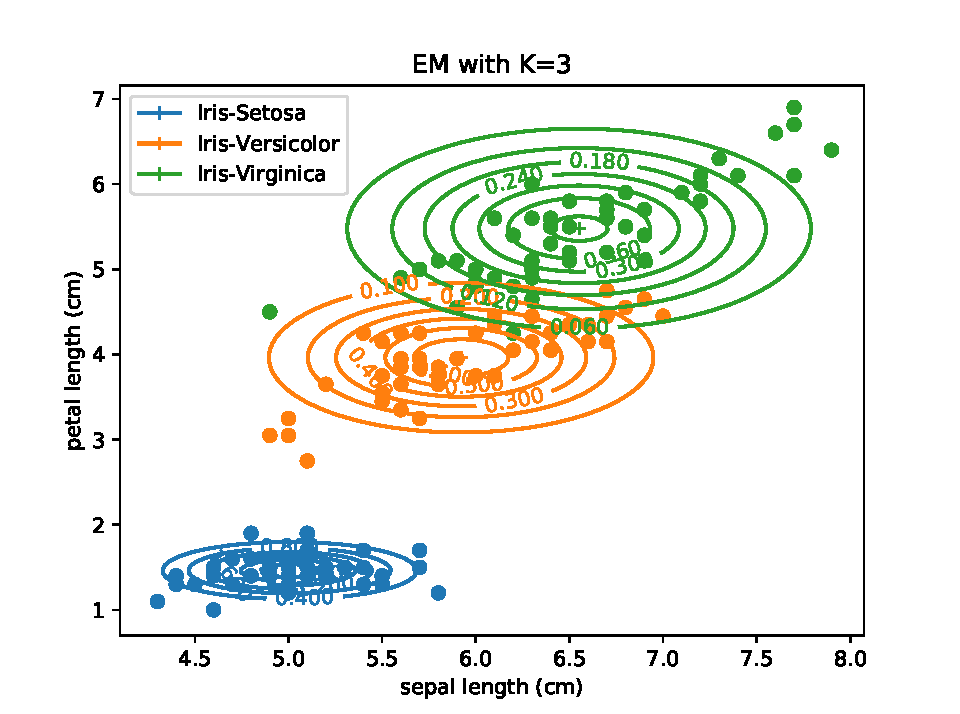
\includegraphics[width=\textwidth]{./Figures/2_2_EM_cont_K3}
	%\caption{$K=3$}
	\end{subfigure}
	\begin{subfigure}{0.6\textwidth}
	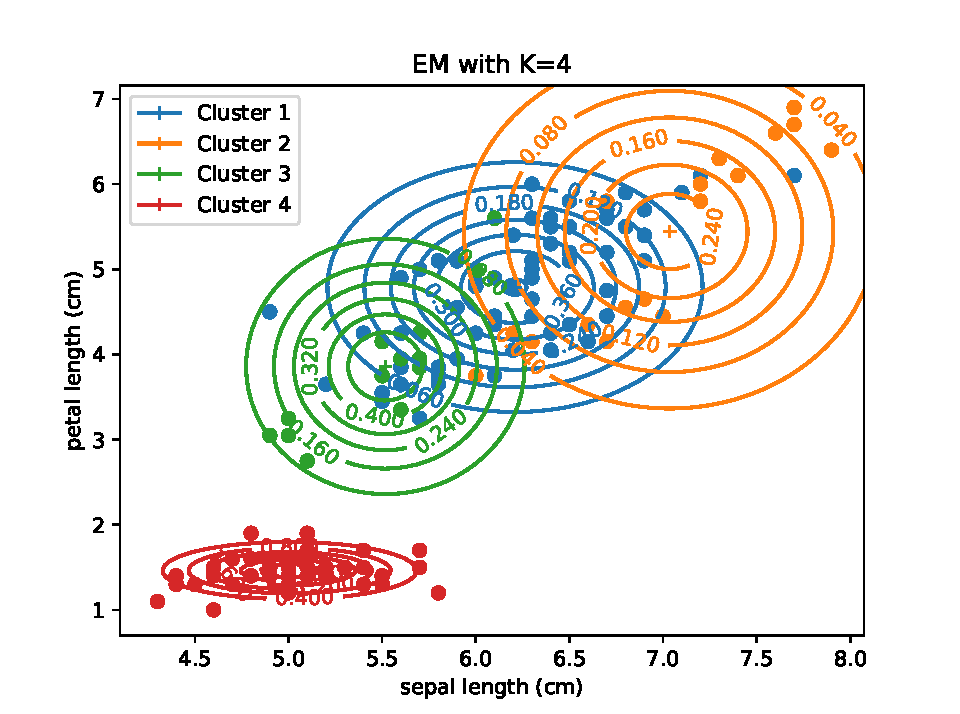
\includegraphics[width=\textwidth]{./Figures/2_2_EM_cont_K4}
	%\caption{$K=4$}
	\end{subfigure}
	}	
	\caption{Results of EM classification with $K=2\dots4$ components.}
	\label{2_2_EM_cont}
\end{figure}

\begin{figure}[!ht]
\centering
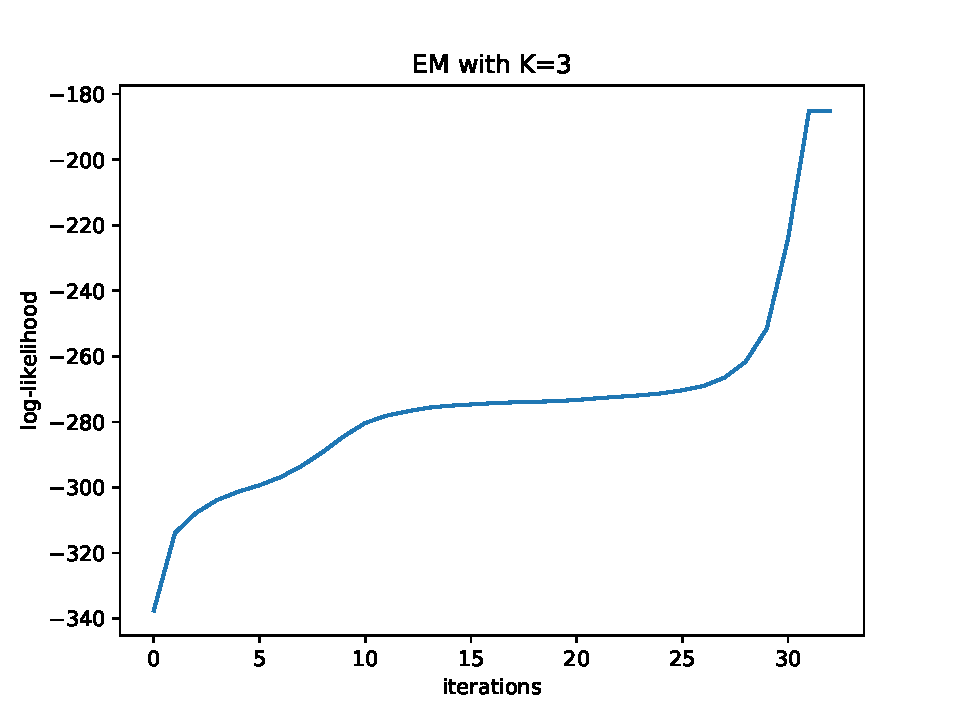
\includegraphics[width=0.6\textwidth]{./Figures/2_2_EM_likelihood_K3}
\caption{Log-likelihood function over iterations for $K=3$ components.}
\label{2_2_EM_likelihood}
\end{figure}

\begin{figure}[!ht]
	\makebox[\textwidth]{
	\begin{subfigure}{0.6\textwidth}
	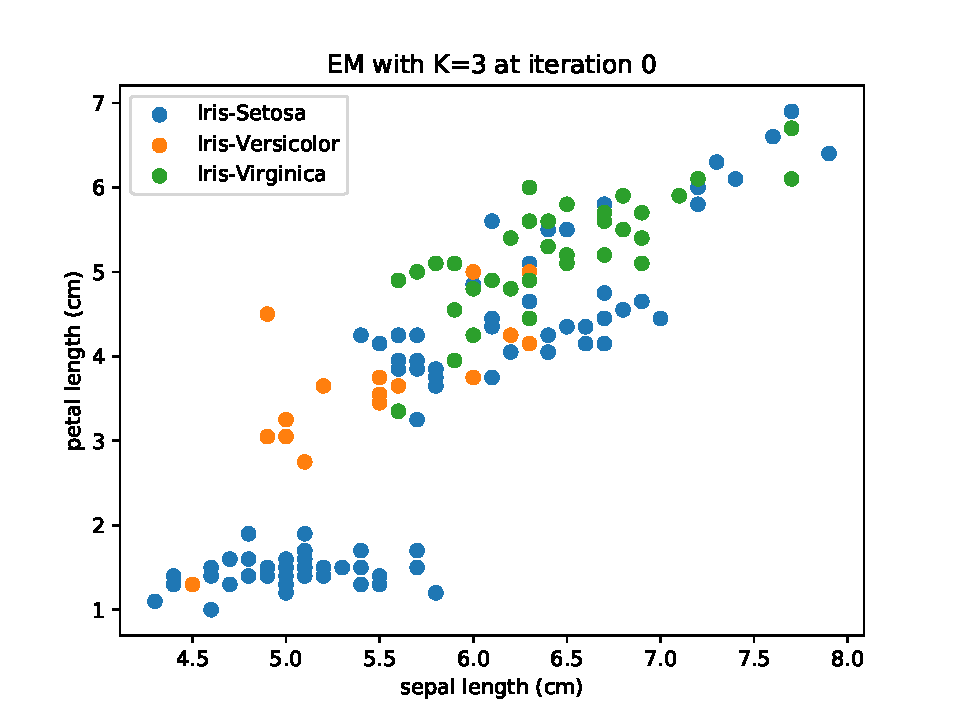
\includegraphics[width=\textwidth]{./Figures/2_2_EM_iter0}
	%\caption{Dataset}
	\end{subfigure}
	\begin{subfigure}{0.6\textwidth}
	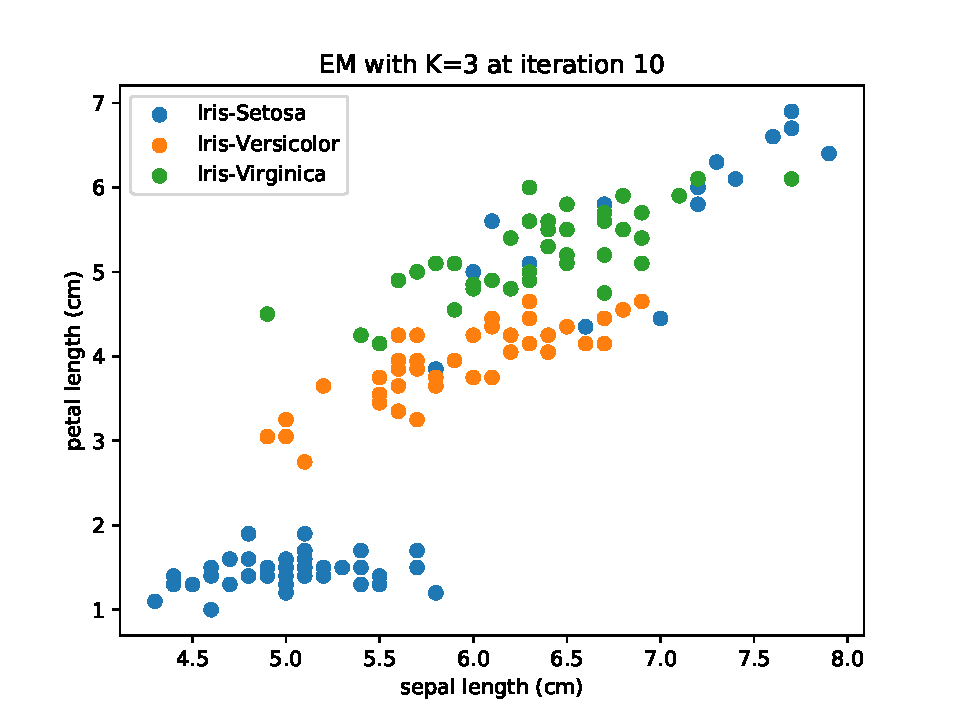
\includegraphics[width=\textwidth]{./Figures/2_2_EM_iter10}
	%\caption{$K=2$}
	\end{subfigure}
	}
	\makebox[\textwidth]{
	\begin{subfigure}{0.6\textwidth}
	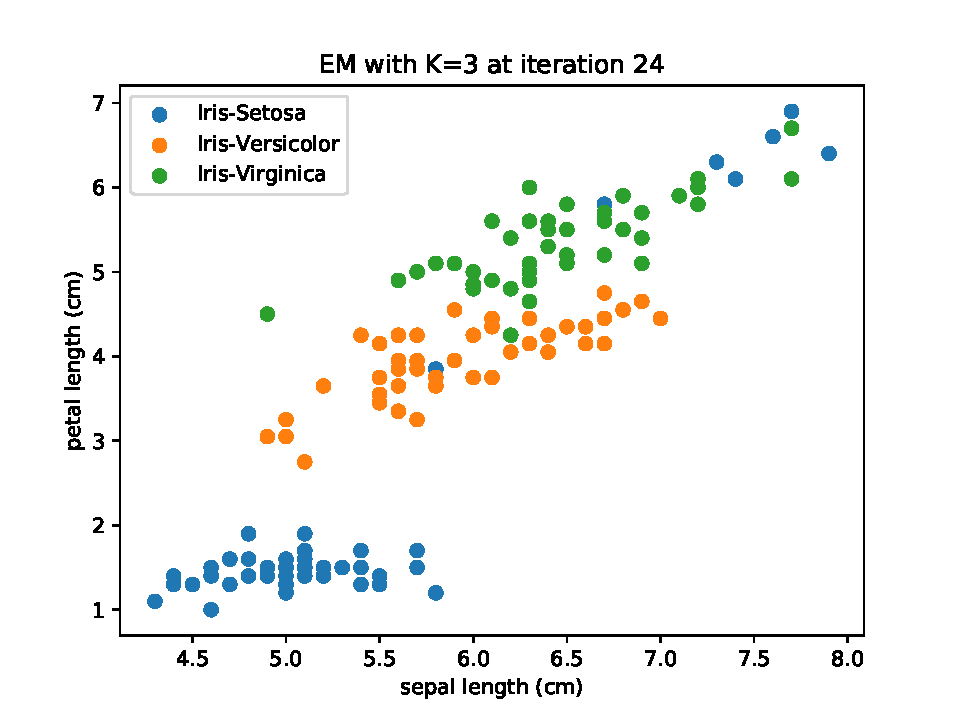
\includegraphics[width=\textwidth]{./Figures/2_2_EM_iter24}
	%\caption{$K=3$}
	\end{subfigure}
	\begin{subfigure}{0.6\textwidth}
	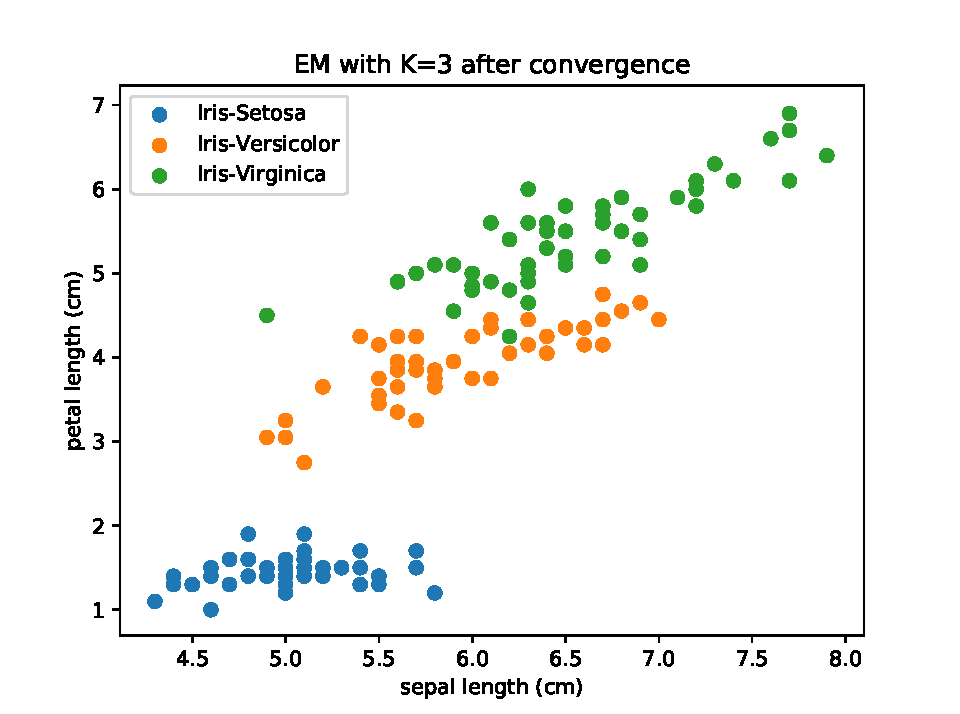
\includegraphics[width=\textwidth]{./Figures/2_2_EM_converged}
	%\caption{$K=4$}
	\end{subfigure}
	}	
	\caption{Results of soft-classification done in E-step.}
	\label{2_2_EM_iter}
\end{figure}


\begin{figure}[!ht]
	\makebox[\textwidth]{
	\begin{subfigure}{0.6\textwidth}
	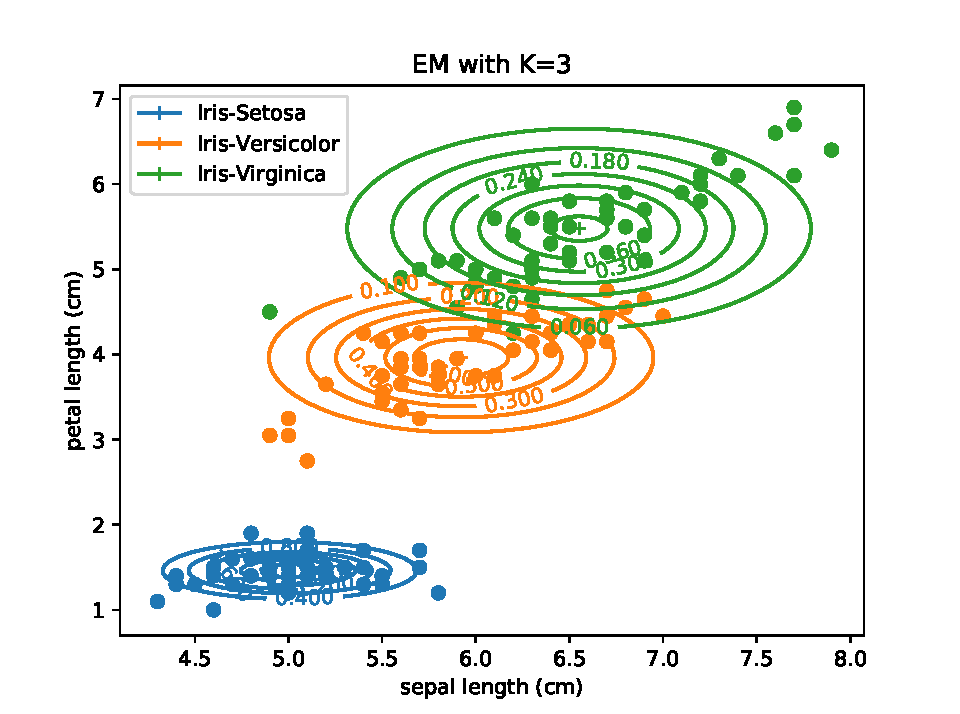
\includegraphics[width=\textwidth]{./Figures/2_2_EM_cont_K3}
	%\caption{Dataset}
	\end{subfigure}
	\begin{subfigure}{0.6\textwidth}
	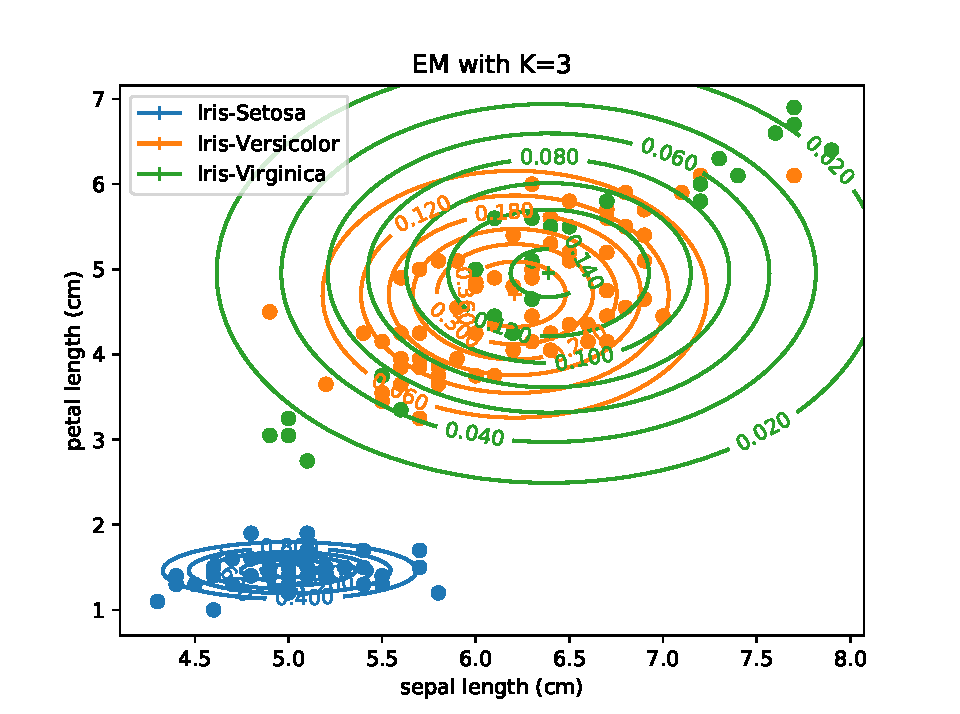
\includegraphics[width=\textwidth]{./Figures/2_2_EM_randinit1}
	%\caption{$K=2$}
	\end{subfigure}
	}
	\makebox[\textwidth]{
	\begin{subfigure}{0.6\textwidth}
	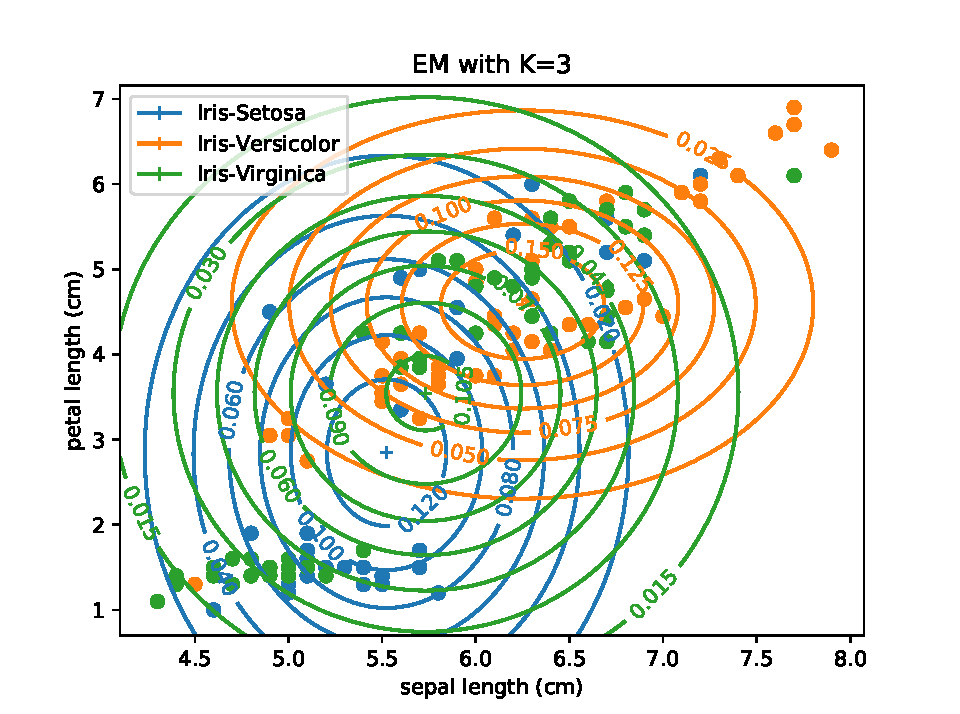
\includegraphics[width=\textwidth]{./Figures/2_2_EM_randinit2}
	%\caption{$K=3$}
	\end{subfigure}
	\begin{subfigure}{0.6\textwidth}
	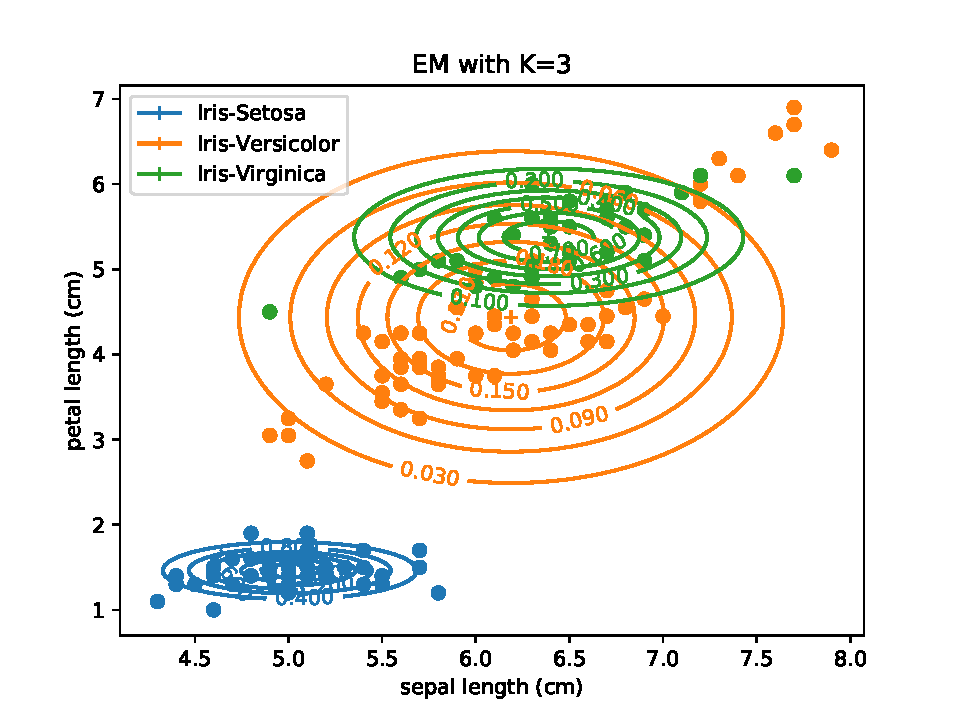
\includegraphics[width=\textwidth]{./Figures/2_2_EM_randinit3}
	%\caption{$K=4$}
	\end{subfigure}
	}	
	\caption{Results of EM classification for several random \texttt{mean0} starting samples.}
	\label{2_2_EM_rand_init}
\end{figure}

\clearpage

\subsection{EM algorithm with diagonal covariance matrices}

\begin{figure}[!ht]
	\makebox[\textwidth]{
	\begin{subfigure}{0.6\textwidth}
	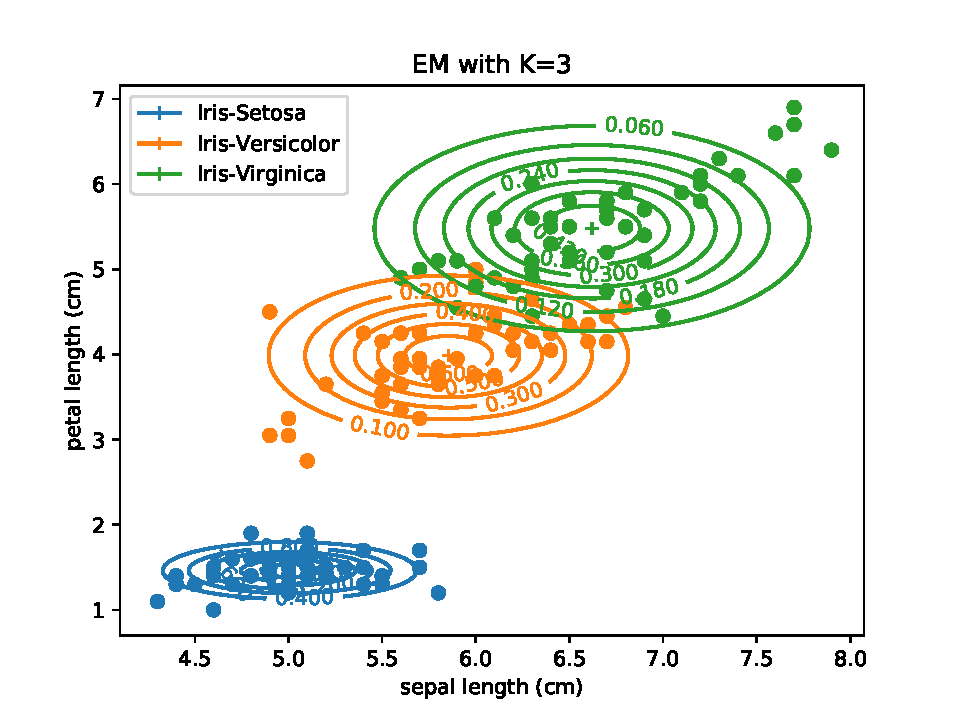
\includegraphics[width=\textwidth]{./Figures/2_2_diagonal_contour_K3}
	\caption{Results of classification}
	\end{subfigure}
	\begin{subfigure}{0.6\textwidth}
	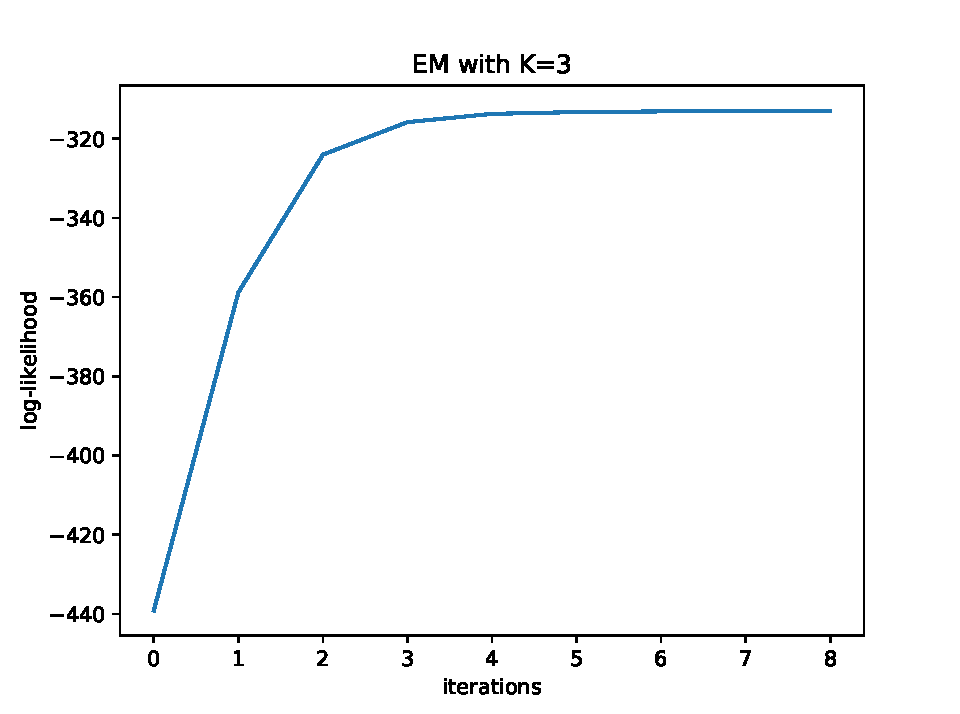
\includegraphics[width=\textwidth]{./Figures/2_2_diagonal_likelihood_K3}
	\caption{Log-likelihood}
	\end{subfigure}
	}
	\caption{Results of EM classification with diagonal covariance matrices.}
	\label{2_2_diagonal}
\end{figure}

\clearpage

\subsection{K-means algorithm}

\begin{figure}[!ht]
	\makebox[\textwidth]{
	\begin{subfigure}{0.6\textwidth}
	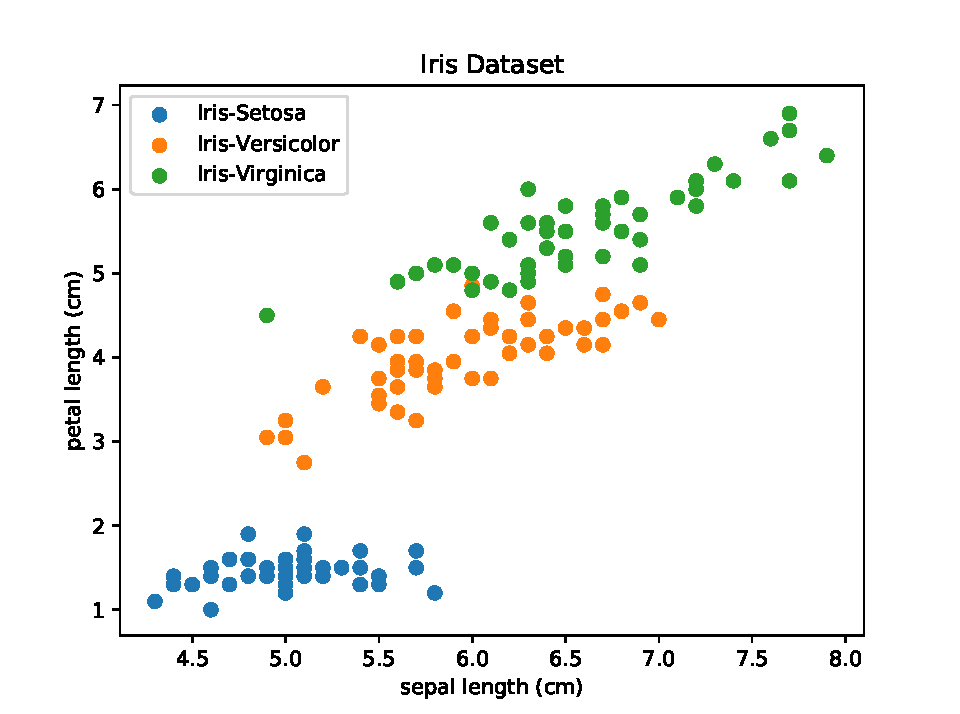
\includegraphics[width=\textwidth]{./Figures/data}
	%\caption{Dataset}
	\end{subfigure}
	\begin{subfigure}{0.6\textwidth}
	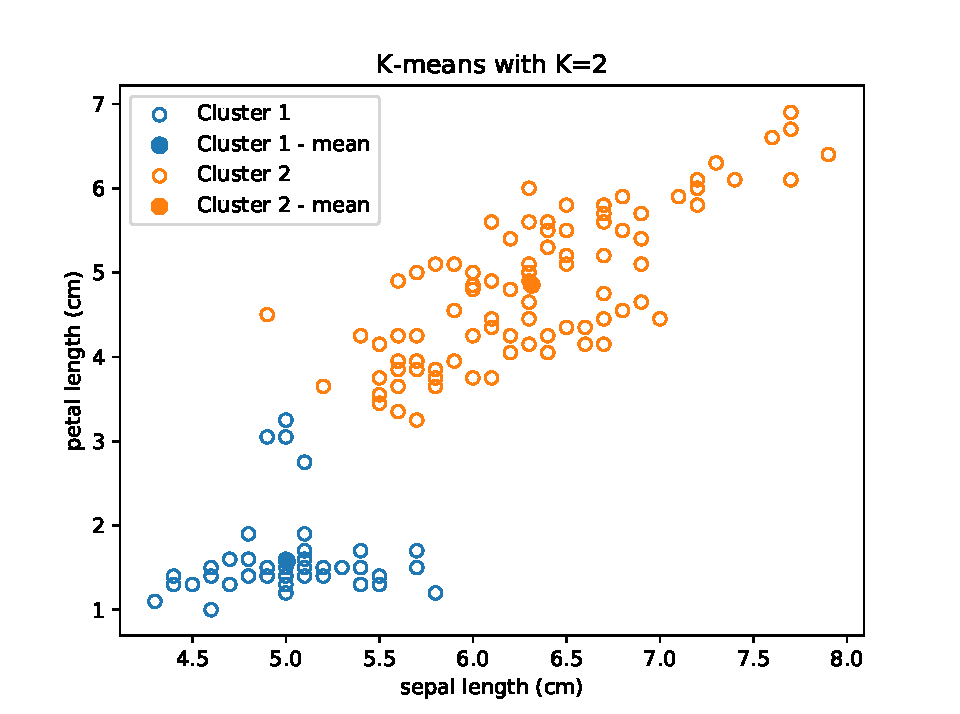
\includegraphics[width=\textwidth]{./Figures/2_2_Kmeans_scatter_K2}
	%\caption{$K=2$}
	\end{subfigure}
	}
	\makebox[\textwidth]{
	\begin{subfigure}{0.6\textwidth}
	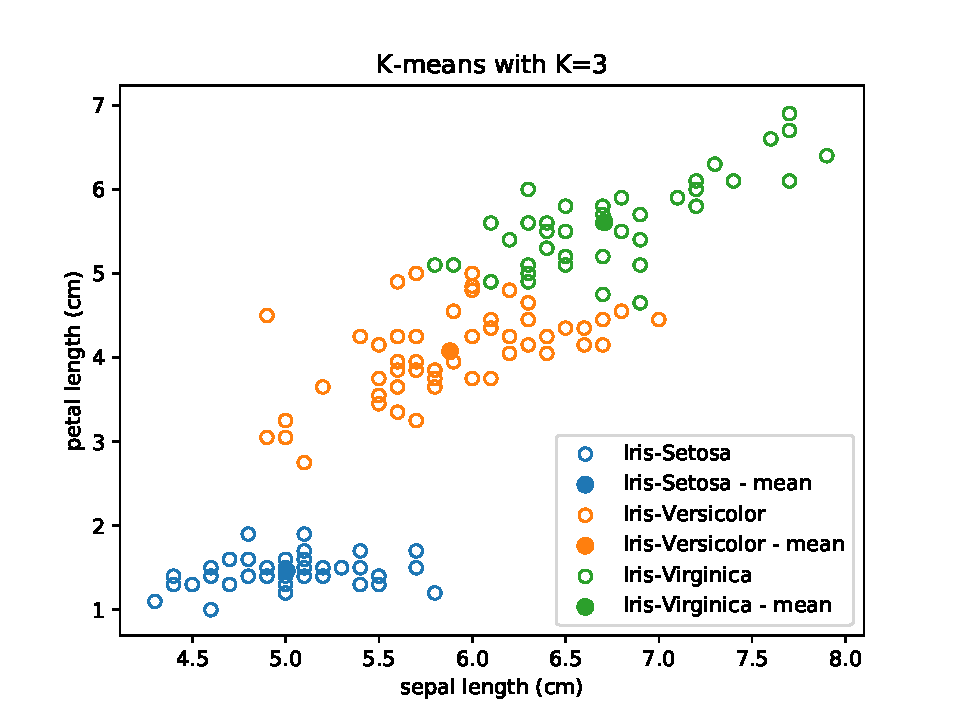
\includegraphics[width=\textwidth]{./Figures/2_2_Kmeans_scatter_K3}
	%\caption{$K=3$}
	\end{subfigure}
	\begin{subfigure}{0.6\textwidth}
	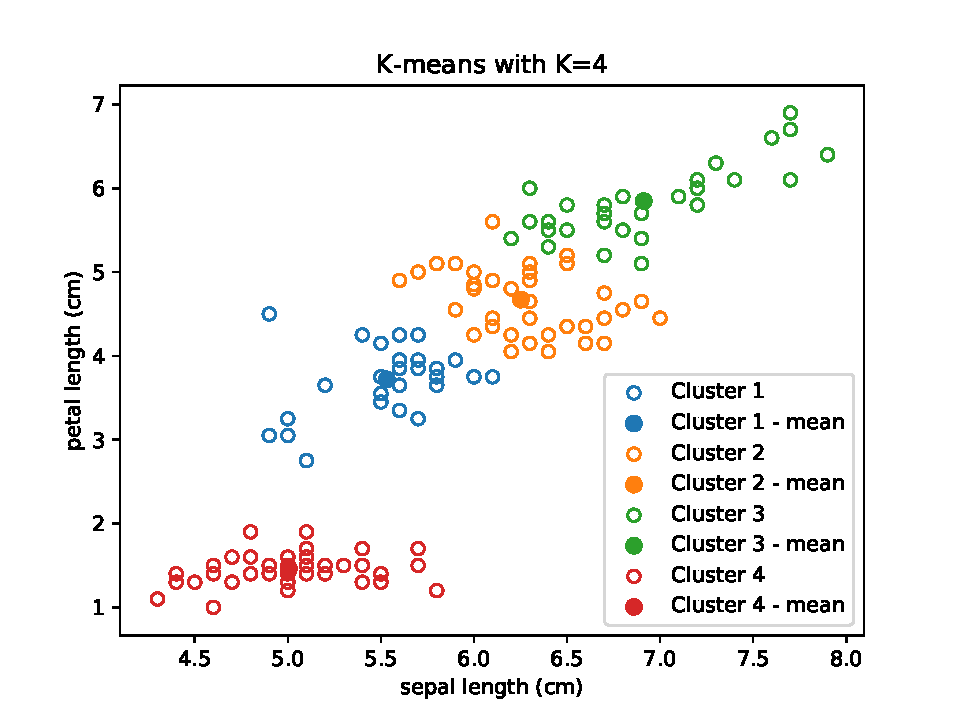
\includegraphics[width=\textwidth]{./Figures/2_2_Kmeans_scatter_K4}
	%\caption{$K=4$}
	\end{subfigure}
	}	
	\caption{Results of K-means classification with $K=2\dots4$ components.}
	\label{2_2_Kmeans_scatter}
\end{figure}\\

Using four features the K-mean algorithms becomes less prone to outliers. 

\begin{figure}[!ht]
\centering
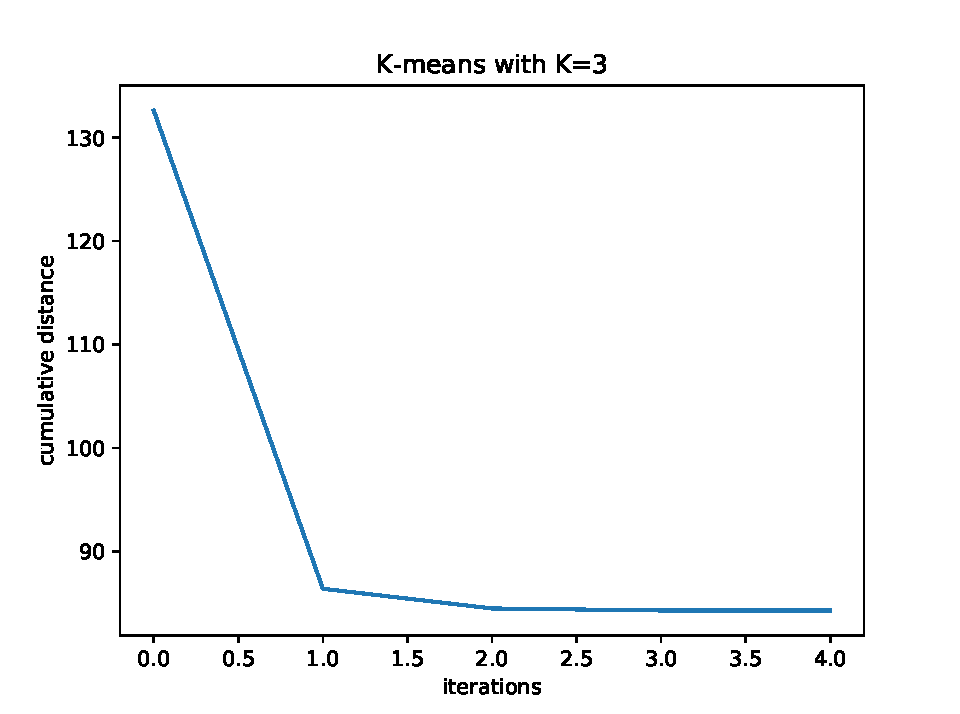
\includegraphics[width=0.6\textwidth]{./Figures/2_2_Kmeans_distance_K3}
\caption{Cumulative distance function over iterations for $K=3$ components.}
\label{2_2_Kmeans_distance}
\end{figure}

\begin{figure}[!ht]
	\makebox[\textwidth]{
	\begin{subfigure}{0.6\textwidth}
	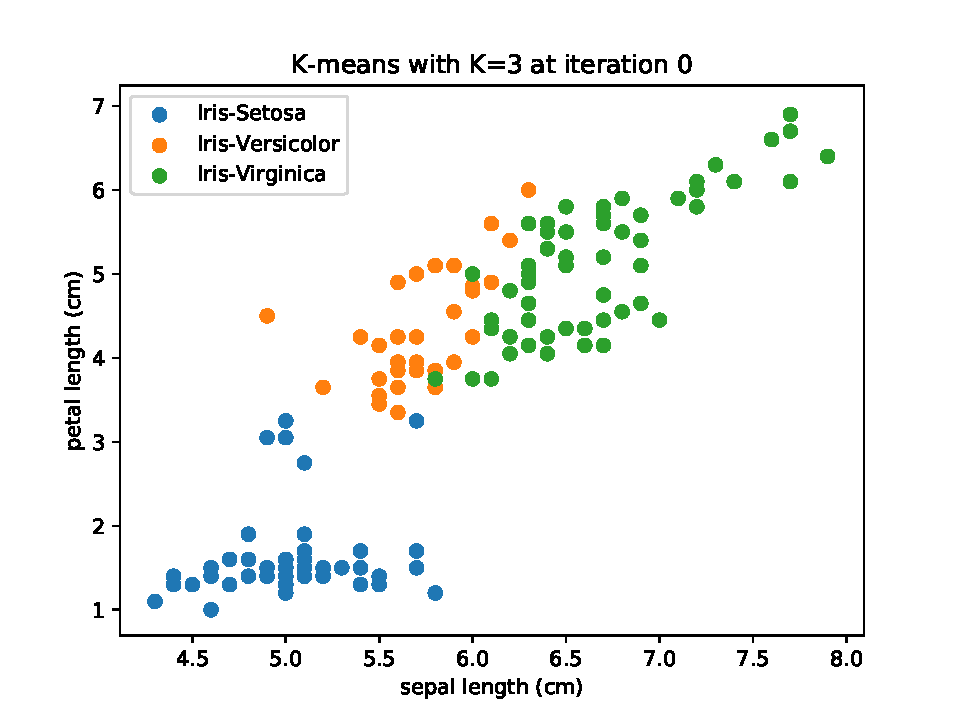
\includegraphics[width=\textwidth]{./Figures/2_2_Kmeans_iter0}
	%\caption{Dataset}
	\end{subfigure}
	\begin{subfigure}{0.6\textwidth}
	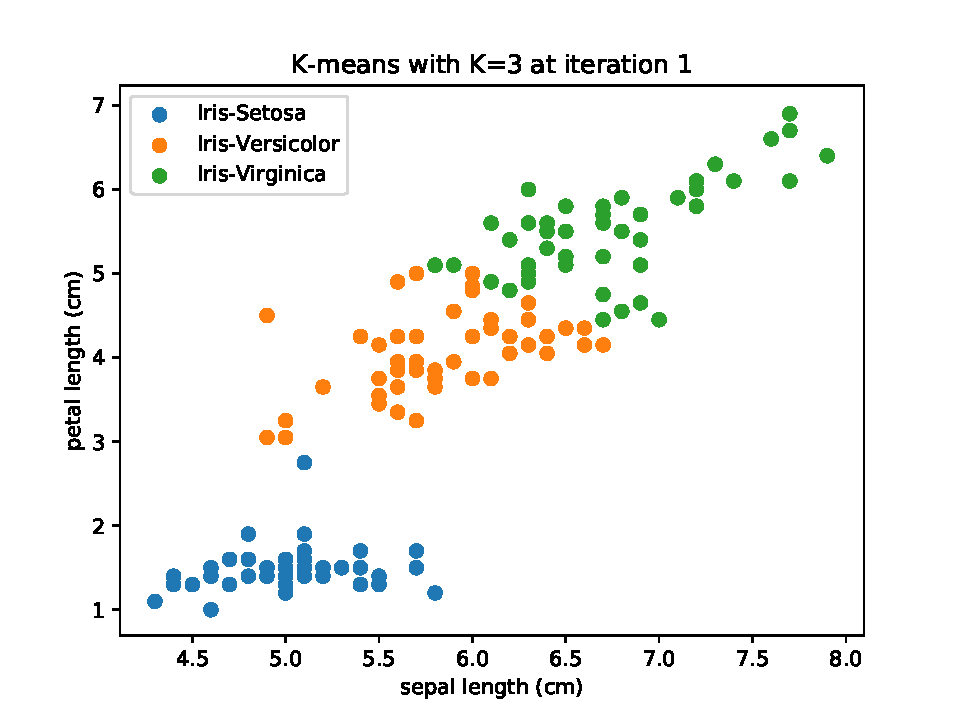
\includegraphics[width=\textwidth]{./Figures/2_2_Kmeans_iter1}
	%\caption{$K=2$}
	\end{subfigure}
	}
	\makebox[\textwidth]{
	\begin{subfigure}{0.6\textwidth}
	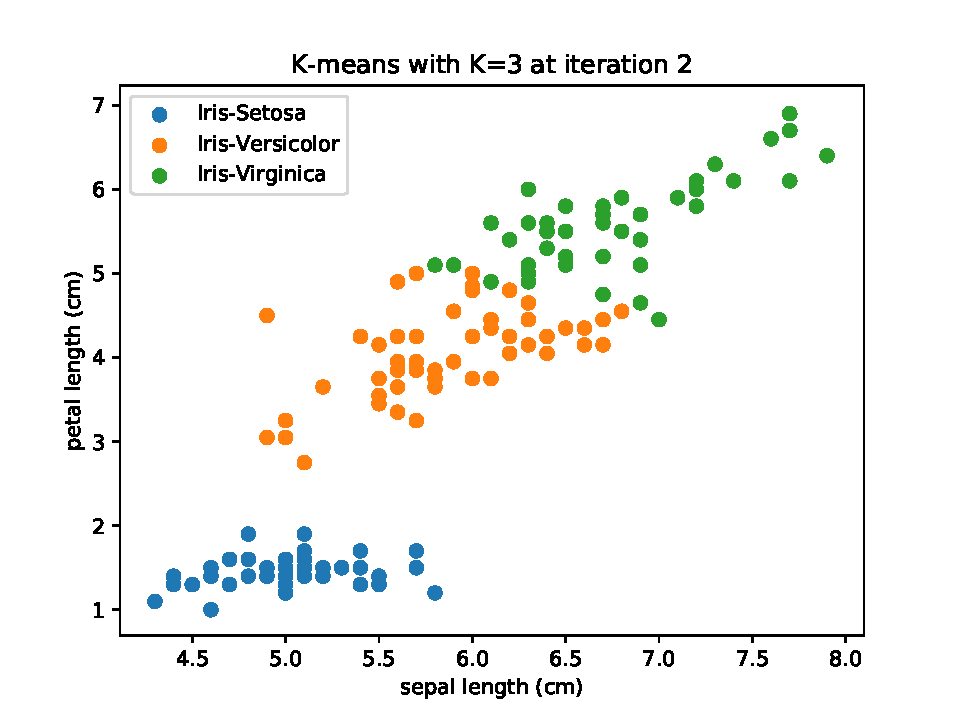
\includegraphics[width=\textwidth]{./Figures/2_2_Kmeans_iter2}
	%\caption{$K=3$}
	\end{subfigure}
	\begin{subfigure}{0.6\textwidth}
	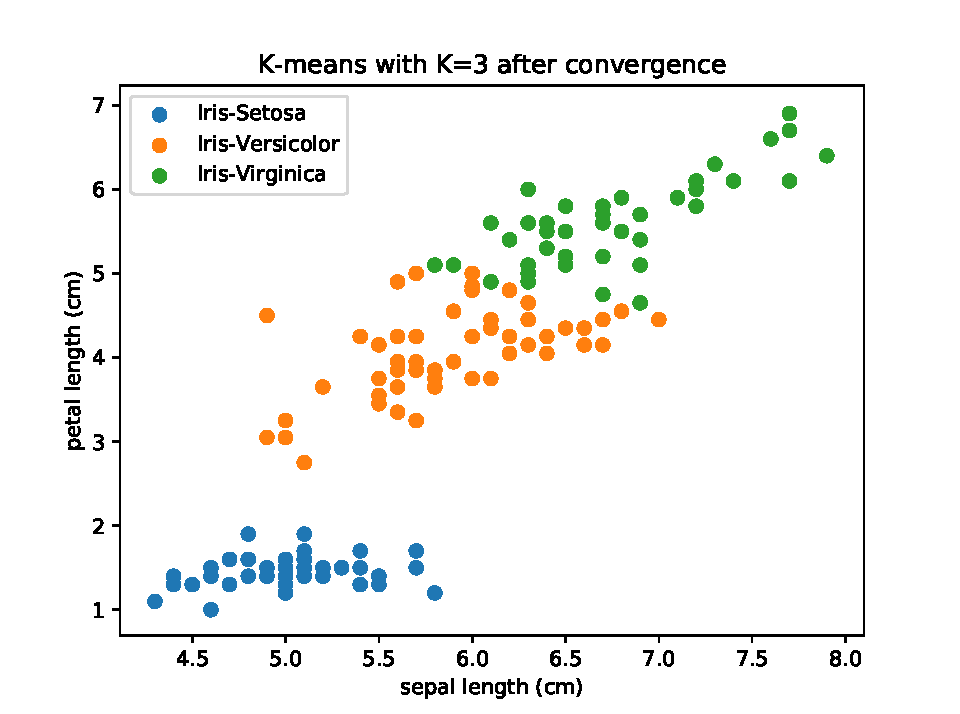
\includegraphics[width=\textwidth]{./Figures/2_2_Kmeans_converged}
	%\caption{$K=4$}
	\end{subfigure}
	}	
	\caption{Results of hard-classification during optimisation.}
	\label{2_2_Kmeans_iter}
\end{figure}


\begin{figure}[!ht]
	\makebox[\textwidth]{
	\begin{subfigure}{0.6\textwidth}
	\includegraphics[width=\textwidth]{./Figures/2_2_Kmeans_scatter_K3}
	%\caption{Dataset}
	\end{subfigure}
	\begin{subfigure}{0.6\textwidth}
	\includegraphics[width=\textwidth]{./Figures/2_2_Kmeans_randinit1}
	%\caption{$K=2$}
	\end{subfigure}
	}
	\makebox[\textwidth]{
	\begin{subfigure}{0.6\textwidth}
	\includegraphics[width=\textwidth]{./Figures/2_2_Kmeans_randinit2}
	%\caption{$K=3$}
	\end{subfigure}
	\begin{subfigure}{0.6\textwidth}
	\includegraphics[width=\textwidth]{./Figures/2_2_Kmeans_randinit3}
	%\caption{$K=4$}
	\end{subfigure}
	}	
	\caption{Results of K-means classification for several random \texttt{center0} starting samples.}
	\label{2_2_Kmeans_randinit}
\end{figure}

\end{document}}